\documentclass[a4paper, 11pt, parskip=half, headsepline]{scrreprt}

\usepackage{scrlayer-scrpage}                   % Headings
\usepackage{txfontsb}                           % Default font
\usepackage{sourcecodepro}                      % Monospace font
\usepackage[utf8]{inputenc}                     % Input encoding
\usepackage[T1]{fontenc}                        % Output encoding
\usepackage{graphicx}                           % Pictures
\usepackage{listings}                           % Code snippets
\usepackage{hyperref}                           % Make strings clickable
\usepackage[usenames,dvipsnames,table]{xcolor}  % Colors
\usepackage[toc,page]{appendix}                 % Support for appendices
\usepackage[chapter]{algorithm}                 % Pseudocode headers
\usepackage{algpseudocode}                      % Pseudocode
\usepackage{pdfpages}                           % Embed external pdf
\usepackage{wrapfig}                            % Wrap text around figures
\usepackage{multicol}                           % Used for multicolumn itemize
\usepackage{multirow}                           % Used for multirow in tables
\usepackage{longtable}                          % Tables can spread over multiple pages
\usepackage{enumerate}                          % Custom item numbers for enumerations
\usepackage[framemethod=tikz]{mdframed}         % Allows defining custom boxed/framed environments
\usepackage{tocloft}                            % TOC spacing
\usepackage{caption}                            % Remove colon from captions




%----------------------------------------------------------------------------------------
%	DOCUMENT SETTINGS
%----------------------------------------------------------------------------------------

\areaset{17cm}{23.5cm}              % Set page width and height
\graphicspath{{./figures/}}         % Set path for figures
\setlength{\cftchapnumwidth}{2em}   % Set chapter numwidth
\setlength{\cftsecnumwidth}{3em}    % Set section numwidth
\setlength{\cftsubsecnumwidth}{4em} % Set subsection numwidth
\hypersetup{linktoc=all}            % Set TOC clickable

\lstset{ 
    belowcaptionskip=\baselineskip,
    aboveskip=\baselineskip,
    breaklines=true,
    frame=l,
    xleftmargin=0.5in,
    showstringspaces=false,
    basicstyle=\footnotesize\ttfamily,
    keywordstyle=\bfseries\color{green!40!black},
    commentstyle=\color{MidnightBlue},
    stringstyle=\color{BrickRed},
    numberstyle=\color{Cyan!50!Black},
    numbers=left,
    tabsize=4
}

\pagestyle{scrheadings}
\ihead{Design Document}
\ohead{Codiglioni, dell'Oglio, Nichelini}


%----------------------------------------------------------------------------------------
%	COMMAND LINE ENVIRONMENT
%----------------------------------------------------------------------------------------

% Usage:
% \begin{commandline}
%	\begin{verbatim}
%		$ ls
%		
%		Applications	Desktop	...
%	\end{verbatim}
% \end{commandline}

\mdfdefinestyle{commandline}{
	leftmargin=10pt,
	rightmargin=10pt,
	innerleftmargin=15pt,
	middlelinecolor=black!50!white,
	middlelinewidth=2pt,
	frametitlerule=false,
	backgroundcolor=black!5!white,
	frametitle={Command line},
	frametitlefont={\normalfont\ttfamily\color{white}\hspace{-1em}},
	frametitlebackgroundcolor=black!50!white,
	nobreak,
}

% Define a custom environment for command-line snapshots
\newenvironment{commandline}{
	\medskip
	\begin{mdframed}[style=commandline]
	\footnotesize
}{
	\end{mdframed}
	\medskip
}


%----------------------------------------------------------------------------------------
%	FILE CONTENTS ENVIRONMENT
%----------------------------------------------------------------------------------------

% Usage:
% \begin{file}[optional filename, defaults to "File"]
%	File contents, for example, with a listings environment
% \end{file}

\mdfdefinestyle{file}{
	innertopmargin=1.6\baselineskip,
	innerbottommargin=0.28\baselineskip,
	topline=false, bottomline=false,
	leftline=false, rightline=false,
	leftmargin=2cm,
	rightmargin=2cm,
	singleextra={%
		\draw[fill=black!10!white](P)++(0,-1.3em)rectangle(P-|O);
		\node[anchor=north west]
		at(P-|O){\footnotesize\ttfamily\mdfilename};
		%
		\def\l{1.5em}
		\draw(O-|P)++(-\l,0)--++(\l,\l)--(P)--(P-|O)--(O)--cycle;
		\draw(O-|P)++(-\l,0)--++(0,\l)--++(\l,0);
	},
	nobreak,
}

% Define a custom environment for file contents
\newenvironment{file}[1][File]{ % Set the default filename to "File"
	\medskip
	\newcommand{\mdfilename}{#1}
	\begin{mdframed}[style=file]
}{
	\end{mdframed}
	\medskip
}


%----------------------------------------------------------------------------------------
%	NUMBERED QUESTIONS ENVIRONMENT
%----------------------------------------------------------------------------------------

% Usage:
% \begin{question}[optional title]
%	Question contents
% \end{question}

\mdfdefinestyle{question}{
	innertopmargin=1.2\baselineskip,
	innerbottommargin=0.8\baselineskip,
	roundcorner=5pt,
	nobreak,
	singleextra={%
		\draw(P-|O)node[xshift=1em,anchor=west,fill=white,draw,rounded corners=5pt]{%
		Question \theQuestion\questionTitle};
	},
}

\newcounter{Question} % Stores the current question number that gets iterated with each new question

% Define a custom environment for numbered questions
\newenvironment{question}[1][\unskip]{
	\bigskip
	\stepcounter{Question}
	\newcommand{\questionTitle}{~#1}
	\begin{mdframed}[style=question]
}{
	\end{mdframed}
	\medskip
}


%----------------------------------------------------------------------------------------
%	BOXED PARAGRAPH ENVIRONMENT
%----------------------------------------------------------------------------------------

% Usage:
% \begin{boxedpar}[optional title]
%	Question contents
% \end{boxedpar}

\mdfdefinestyle{boxedpar}{
	innertopmargin=1.2\baselineskip,
	innerbottommargin=0.8\baselineskip,
	roundcorner=5pt,
	nobreak,
	singleextra={%
		\draw(P-|O)node[xshift=1em,anchor=west,fill=white,draw,rounded corners=5pt]{%
		\textit{\boxTitle}};
	},
}

% Define a custom environment for numbered questions
\newenvironment{boxedpar}[1][in-depth]{
	\bigskip
	\newcommand{\boxTitle}{#1}
	\begin{mdframed}[style=boxedpar]
}{
	\end{mdframed}
	\medskip
}


%----------------------------------------------------------------------------------------
%	ROUNDED BOX ENVIRONMENT
%----------------------------------------------------------------------------------------

% Usage:
% \begin{roundedbox}
%	Contents
% \end{roundedbox}

\mdfdefinestyle{roundedbox}{
	innertopmargin=0.5\baselineskip,
	innerbottommargin=0.5\baselineskip,
	roundcorner=5pt,
	nobreak,
}

% Define a custom environment for numbered questions
\newenvironment{roundedbox}{
	\bigskip
	\begin{mdframed}[style=roundedbox]
}{
	\end{mdframed}
	\medskip
}


%----------------------------------------------------------------------------------------
%	WARNING TEXT ENVIRONMENT
%----------------------------------------------------------------------------------------

% Usage:
% \begin{warn}[optional title, defaults to "Warning:"]
%	Contents
% \end{warn}

\mdfdefinestyle{warning}{
	topline=false, bottomline=false,
	leftline=false, rightline=false,
	nobreak,
	singleextra={%
		\draw(P-|O)++(-0.5em,0)node(tmp1){};
		\draw(P-|O)++(0.5em,0)node(tmp2){};
		\fill[black,rotate around={45:(P-|O)}](tmp1)rectangle(tmp2);
		\node at(P-|O){\color{white}\scriptsize\textbf !};
		\draw[very thick](P-|O)++(0,-1em)--(O);%--(O-|P);
	}
}

% Define a custom environment for warning text
\newenvironment{warn}[1][Warning:]{ % Set the default warning to "Warning:"
	\medskip
	\begin{mdframed}[style=warning]
		\noindent{\textbf{#1}}
}{
	\end{mdframed}
}


%----------------------------------------------------------------------------------------
%	INFORMATION ENVIRONMENT
%----------------------------------------------------------------------------------------

% Usage:
% \begin{info}[optional title, defaults to "Info:"]
% 	contents
% 	\end{info}

\mdfdefinestyle{info}{%
	topline=false, bottomline=false,
	leftline=false, rightline=false,
	nobreak,
	singleextra={%
		\fill[black](P-|O)circle[radius=0.4em];
		\node at(P-|O){\color{white}\scriptsize\textbf i};
		\draw[very thick](P-|O)++(0,-0.8em)--(O);%--(O-|P);
	}
}

% Define a custom environment for information
\newenvironment{info}[1][Info:]{ % Set the default title to "Info:"
	\medskip
	\begin{mdframed}[style=info]
		\noindent{\textbf{#1}}
}{
	\end{mdframed}
}


%----------------------------------------------------------------------------------------
%	LINEDQUOTE ENVIRONMENT
%----------------------------------------------------------------------------------------

% Usage:
% \begin{linedquote}
% 	contents
% 	\end{linedquote}

\mdfdefinestyle{linedquote}{%
	topline=false, bottomline=false,
	leftline=false, rightline=false,
	nobreak,
	singleextra={%
		\draw[very thick](P-|O)++(0,0)--(O);%--(O-|P);
	}
}

% Define a custom environment
\newenvironment{linedquote}{
	\begin{mdframed}[style=linedquote]
}{
	\end{mdframed}
}


%----------------------------------------------------------------------------------------
%	TITLE PAGE
%----------------------------------------------------------------------------------------

\title{Hypermedia Applications\\Design Document}
\author{Fabio Codiglioni - 10484720\\fabio.codiglioni@mail.polimi.it\\\\Luca dell'Oglio - 10497928\\luca1.delloglio@mail.polimi.it\\\\Alessandro Nichelini - 10497404\\alessandro.nichelini@mail.polimi.it}
\date{April 24$^{th}$, 2020}
\publishers{
    \begin{figure}[t]
        \centering
        
\includegraphics[width=0.45\linewidth, keepaspectratio]{Logo_Politecnico_Milano}
    \end{figure}
}


%----------------------------------------------------------------------------------------
%	DOCUMENT
%----------------------------------------------------------------------------------------

\begin{document}

% Title page and TOC
\pagenumbering{gobble}
\maketitle
%\shipout\null           % Blank page
\pagenumbering{roman}
\tableofcontents
\newpage
\pagenumbering{arabic}

% Body

\chapter{Abstract}
The subject of this document is the design of a website for a voluntary association, specifically a time bank. Section 2 contains the C, L, and P sub-models of the Interactive Dialogue Model (IDM). Section 3 lists 3 possible scenarios of use. Section 4 shows the design in the small for different pages. Finally, Section 5 contains the conceptual and logical database design.

\chapter{Graphical representations}

\section{C-IDM}

\begin{figure}[H]
    \centering
    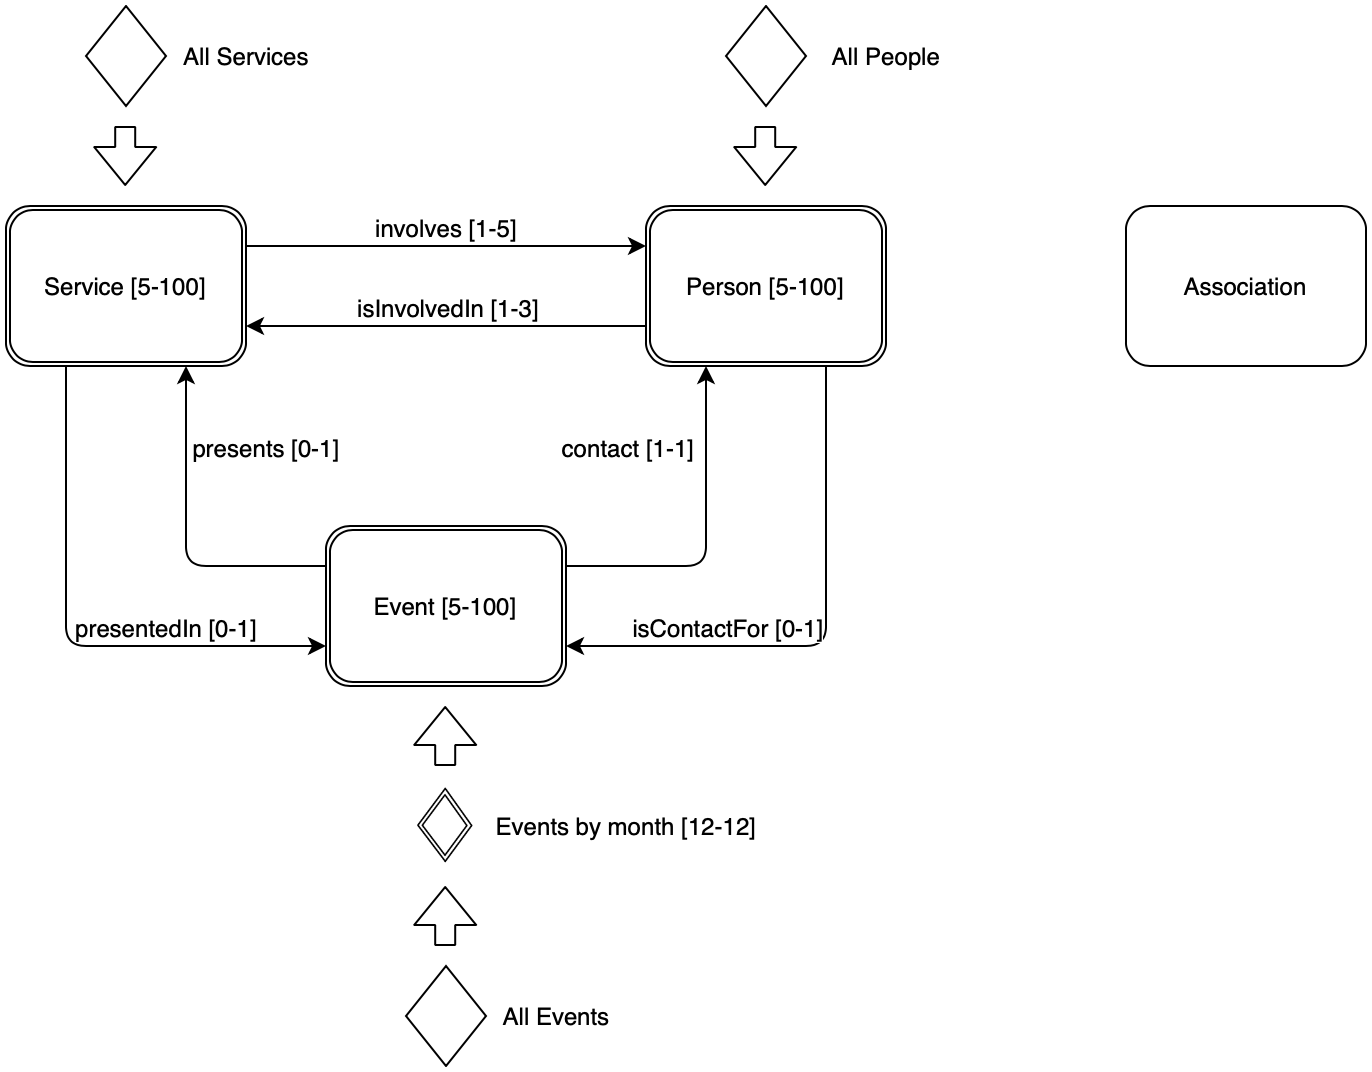
\includegraphics[width=0.85\linewidth, keepaspectratio]{IDM/C-IDM}
\end{figure}

\newpage
\section{L-IDM}

\begin{figure}[H]
    \centering
    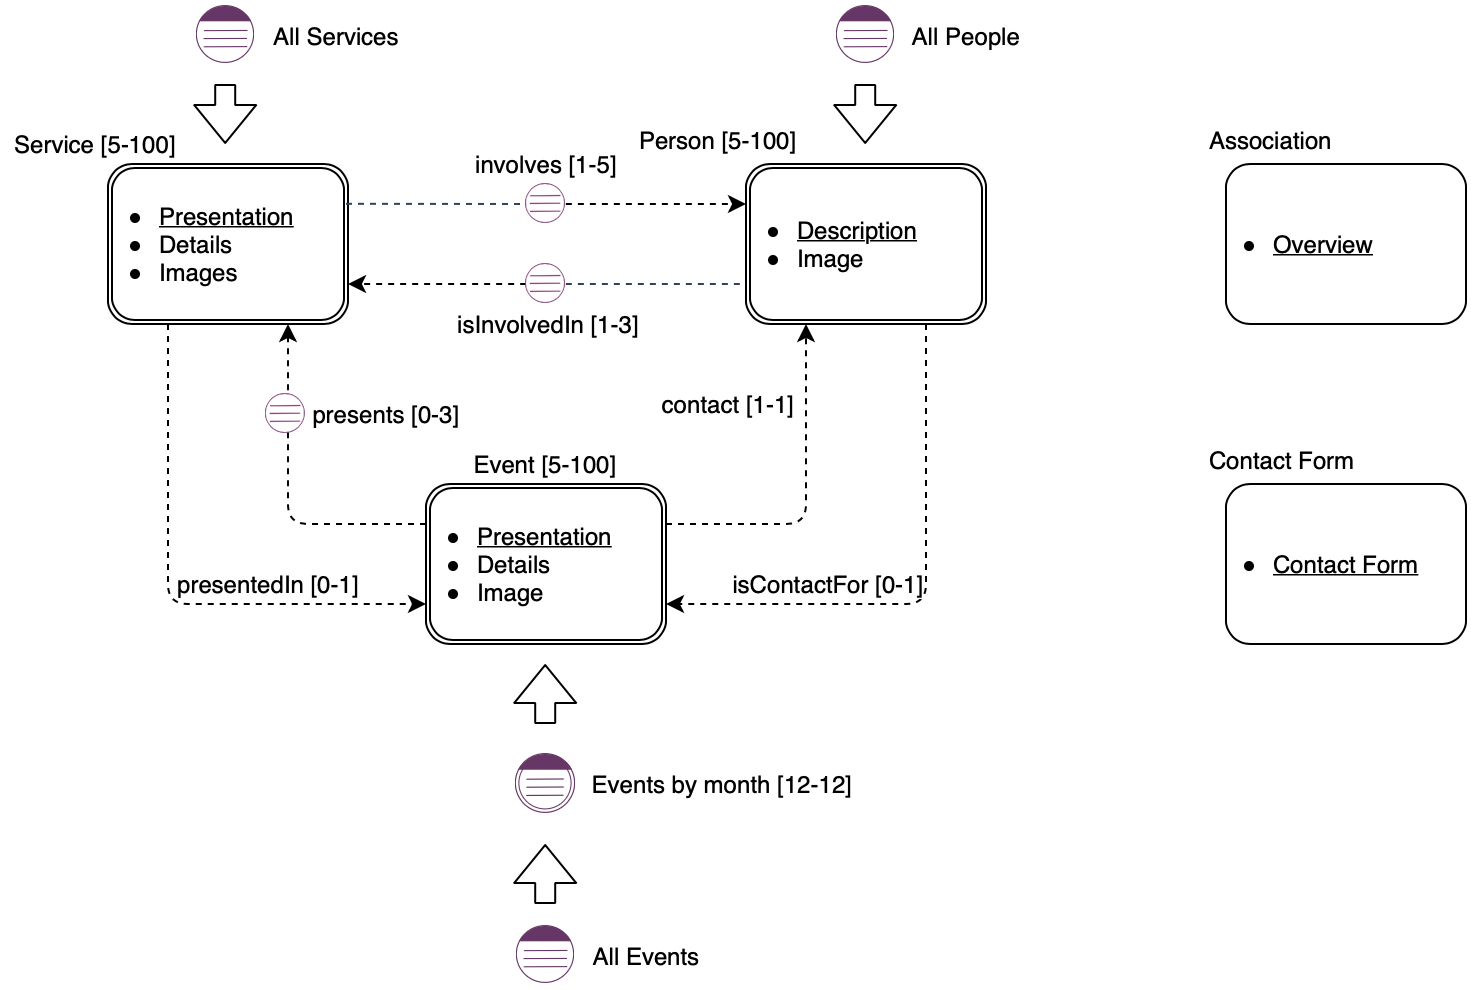
\includegraphics[width=1\linewidth, keepaspectratio]{IDM/L-IDM}
\end{figure}

\newpage
\section{P-IDM}

\begin{figure}[H]
    \centering
    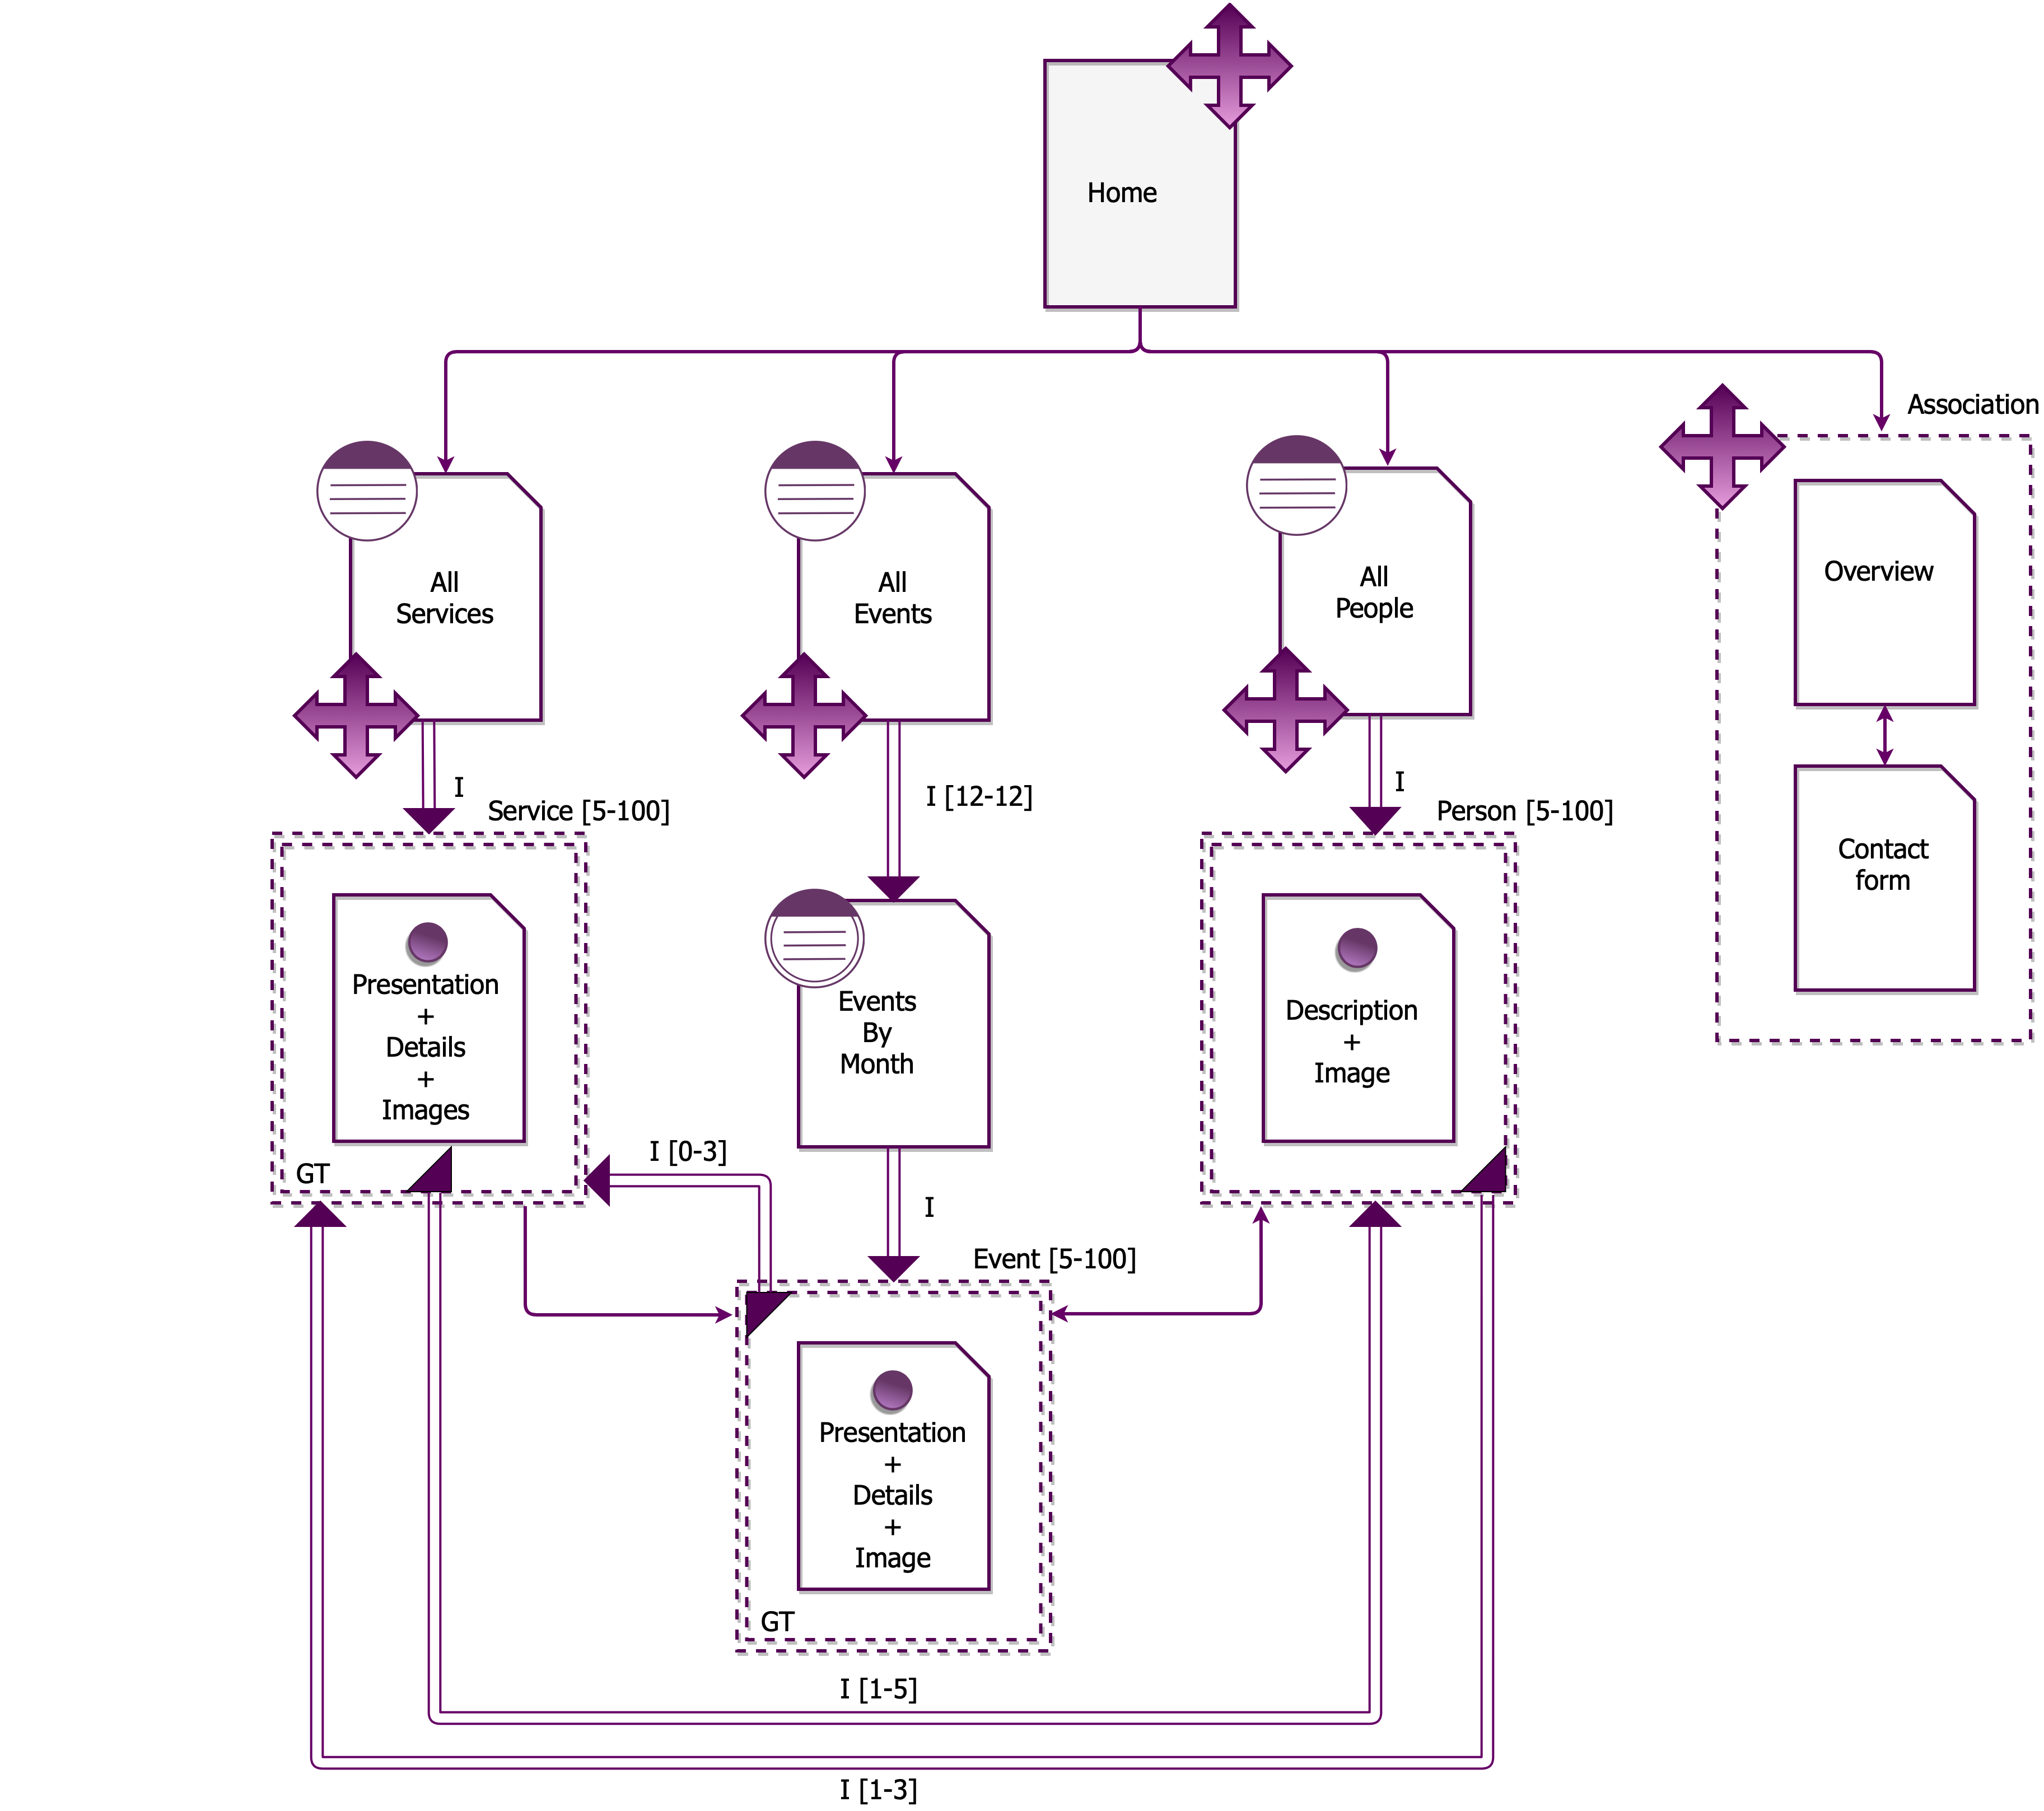
\includegraphics[width=1\linewidth, keepaspectratio]{IDM/P-IDM}
\end{figure}

\chapter{Scenarios}

\section{Scenario 1}

Carol's parents think their daughter needs tutoring for school, so they look for a person who would be able to help her on the time bank website. They open the website and click on the "Services" button on the navigation bar (Figure \ref{fig:scenario-11}). A list of the offered services will be then opened, including the link for the tutoring service (Figure \ref{fig:scenario-12}). After clicking on the link, the parents will see the list of the volunteers that offer tutoring and, by opening the page of one of the volunteers (Figure \ref{fig:scenario-13}), they can see his contact information (Figure \ref{fig:scenario-14}).

\begin{figure}[H]
    \begin{minipage}[t]{0.5\textwidth}
        \centering
    	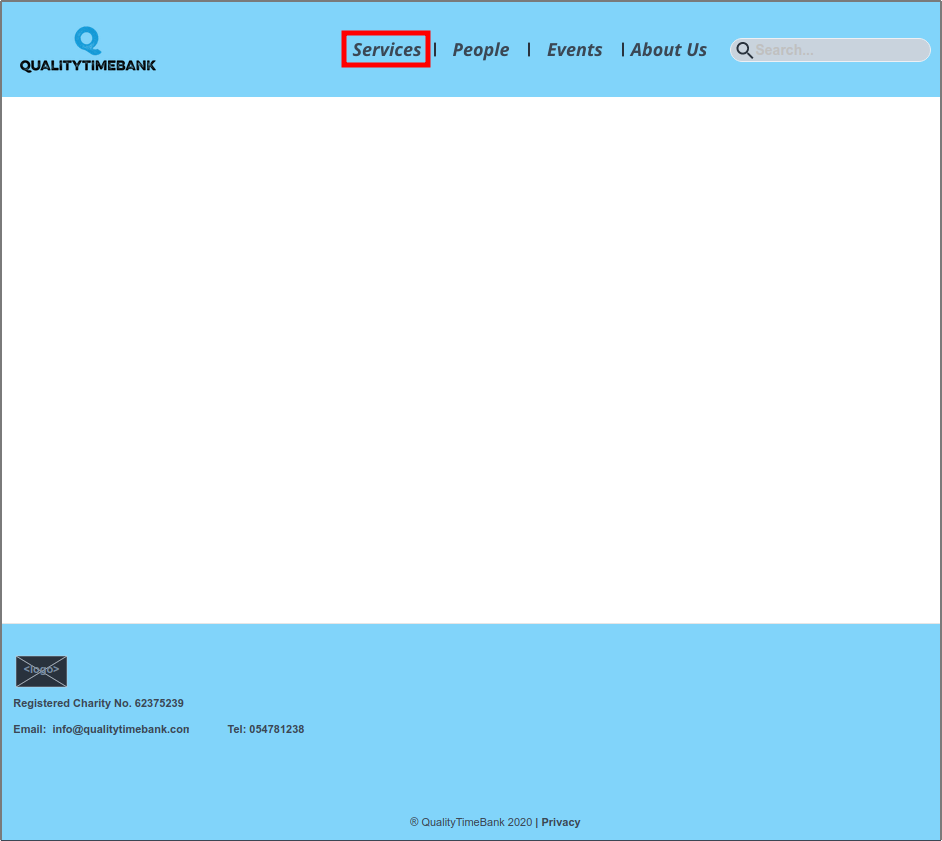
\includegraphics[width=1\linewidth, keepaspectratio]{scenarios/scenario-11}
    	\caption{}
    	\label{fig:scenario-11}
    \end{minipage}
    \hspace*{\fill}
    \begin{minipage}[t]{0.5\textwidth}
        \centering
    	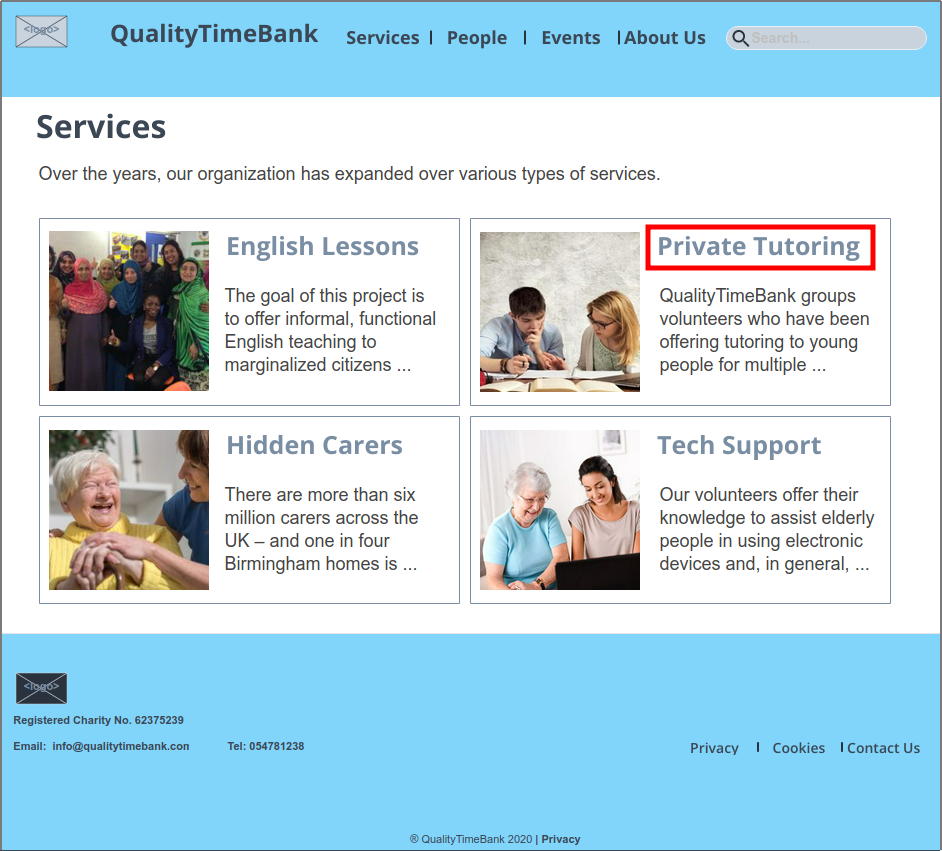
\includegraphics[width=1\linewidth, keepaspectratio]{scenarios/scenario-12}
    	\caption{}
    	\label{fig:scenario-12}
    \end{minipage}
\end{figure}

\begin{figure}[H]
    \begin{minipage}[t]{0.5\textwidth}
        \centering
    	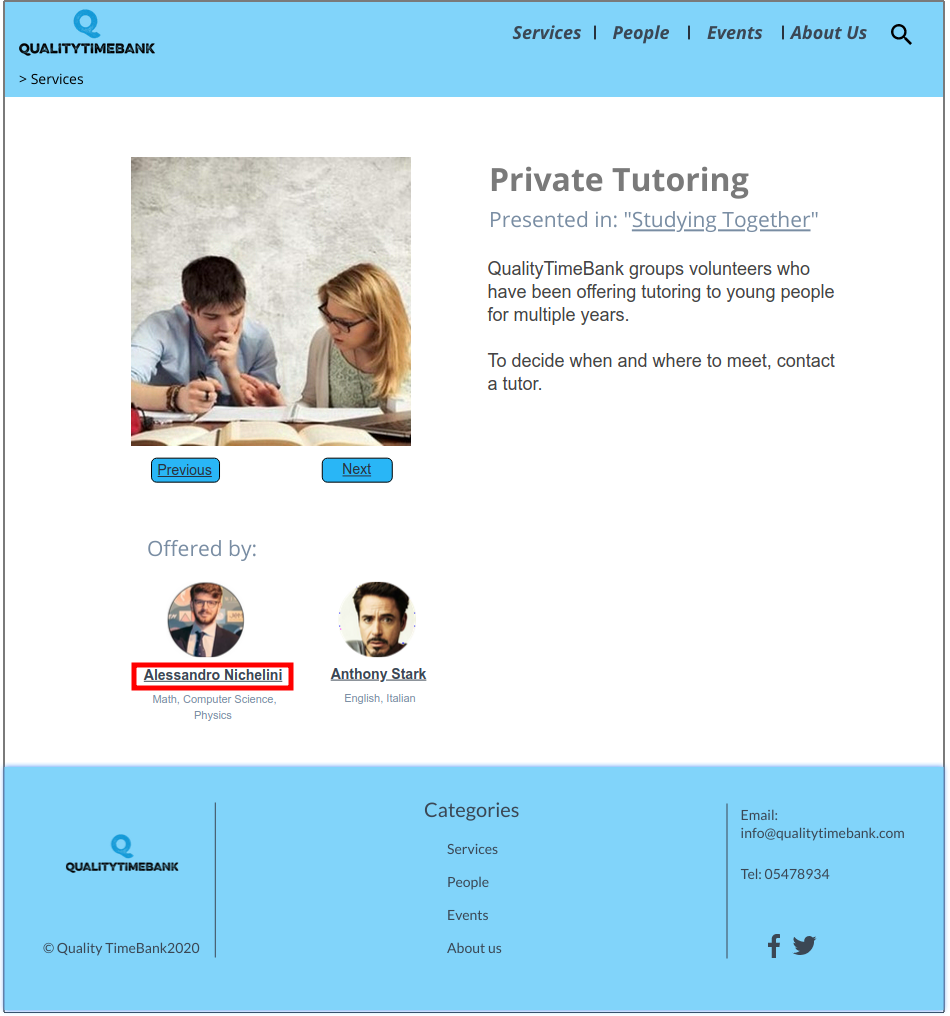
\includegraphics[width=1\linewidth, keepaspectratio]{scenarios/scenario-13}
    	\caption{}
    	\label{fig:scenario-13}
    \end{minipage}
    \hspace*{\fill}
    \begin{minipage}[t]{0.5\textwidth}
        \centering
    	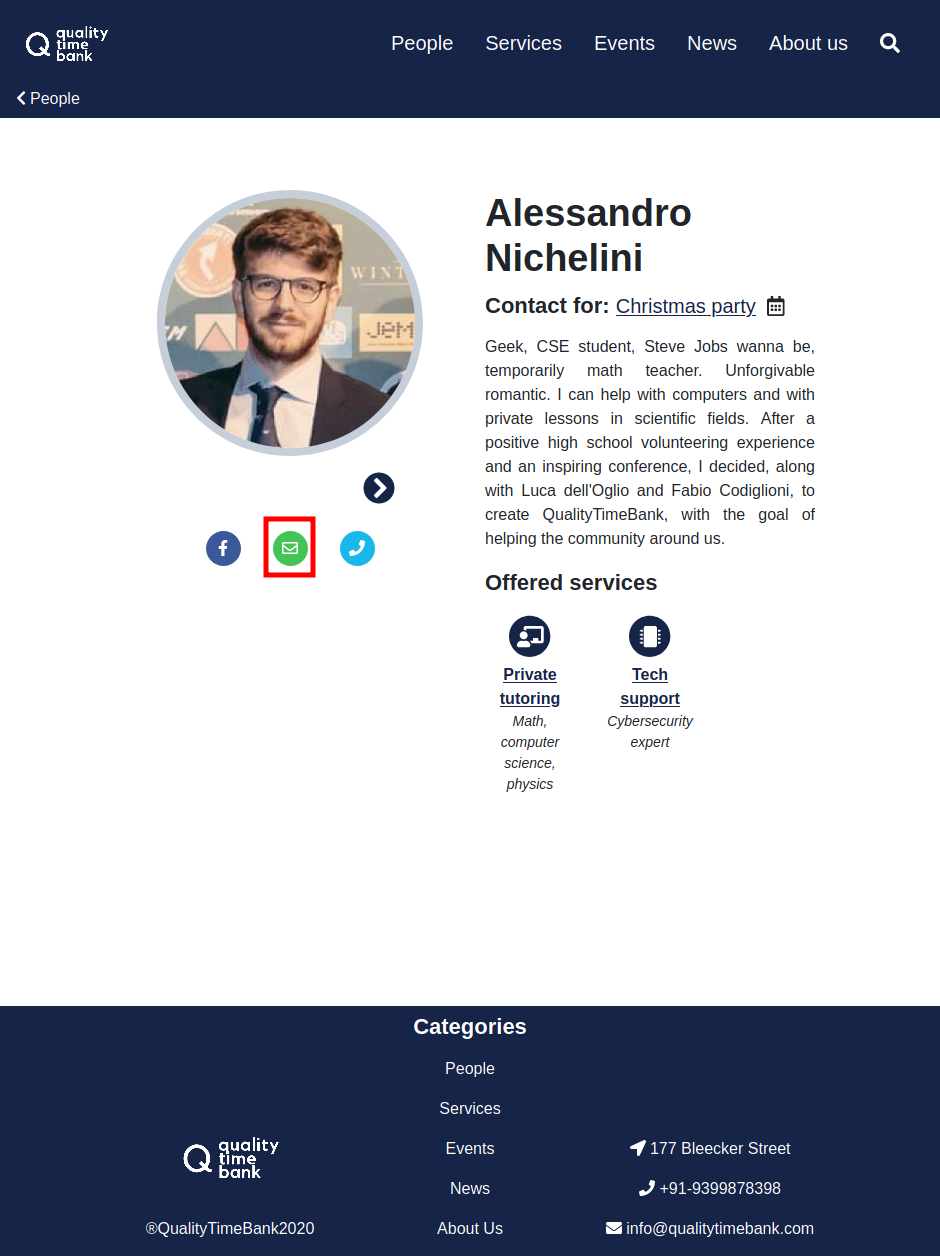
\includegraphics[width=1\linewidth, keepaspectratio]{scenarios/scenario-14}
    	\caption{}
    	\label{fig:scenario-14}
    \end{minipage}
\end{figure}

\section{Scenario 2}	

Giovanni has been an English teacher for the last twenty years, and his New Year's resolution is to share his knowledge with other people. He has heard from a friend that the QualityTimeBank is presenting an English lessons service in January, so he searches the event. By clicking the "Events" button on the home page (Figure \ref{fig:scenario-21}), he reaches the page containing the events of the current month, which is December. By clicking on "January" (Figure \ref{fig:scenario-22}), he reaches the page of that month, where he finds the event he's looking for (Figure \ref{fig:scenario-23}). By clicking on the link, he reaches the page of the event (Figure \ref{fig:scenario-24}).

\begin{figure}[H]
    \begin{minipage}[t]{0.5\textwidth}
        \centering
    	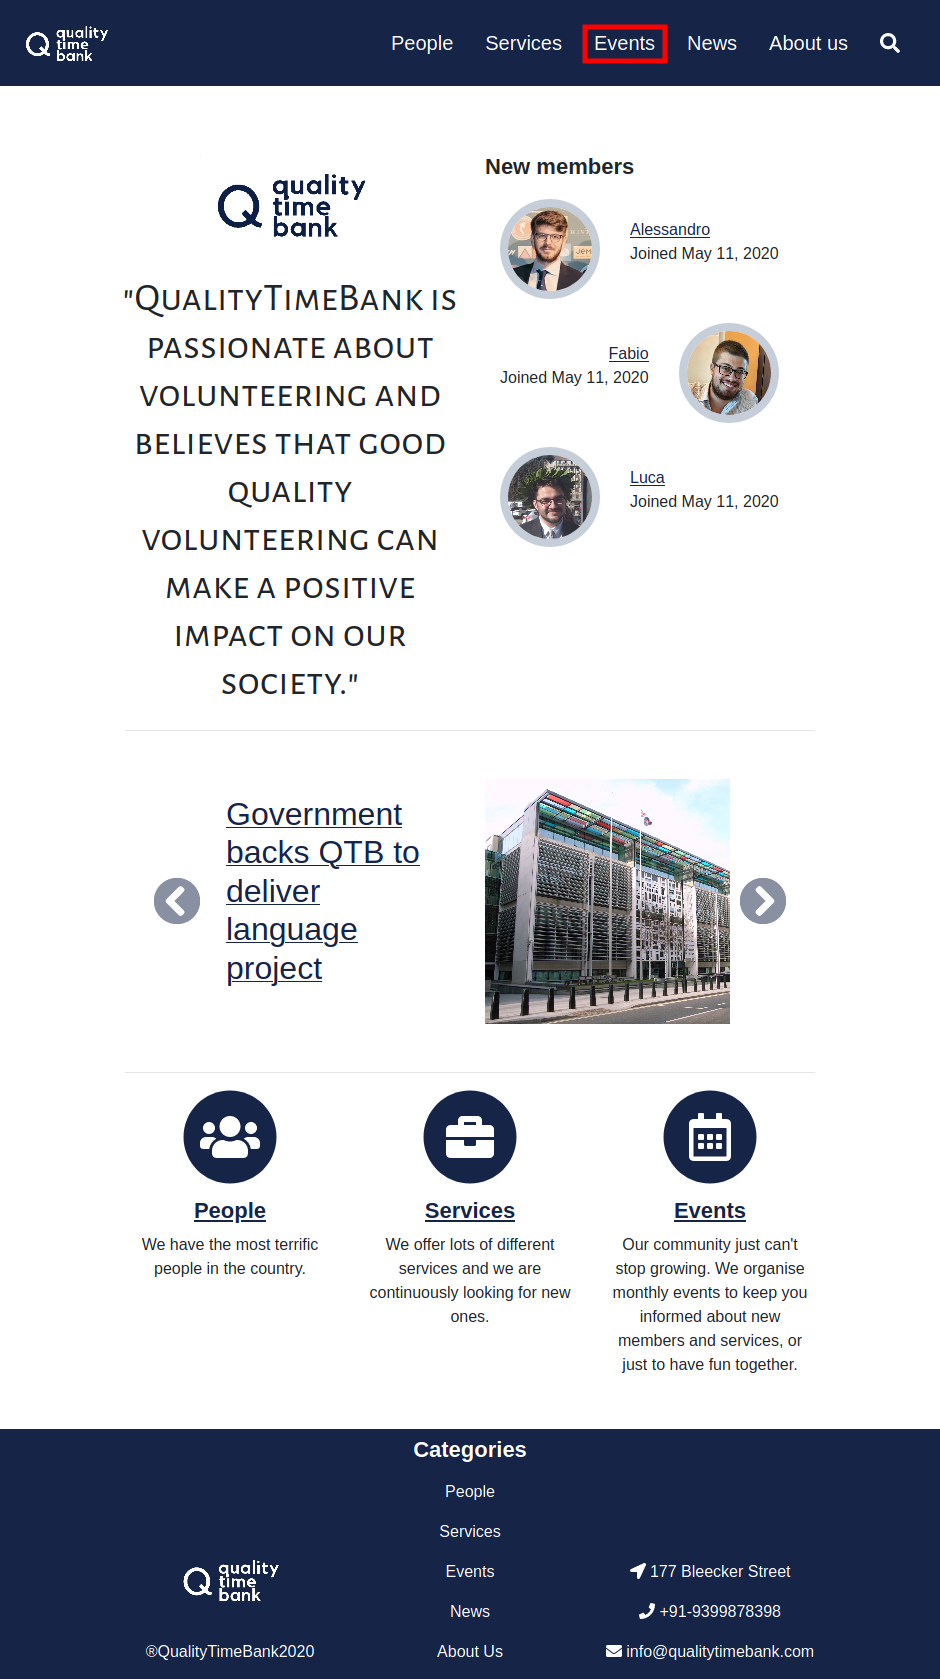
\includegraphics[width=1\linewidth, keepaspectratio]{scenarios/scenario-21}
    	\caption{}
    	\label{fig:scenario-21}
    \end{minipage}
    \hspace*{\fill}
    \begin{minipage}[t]{0.5\textwidth}
        \centering
    	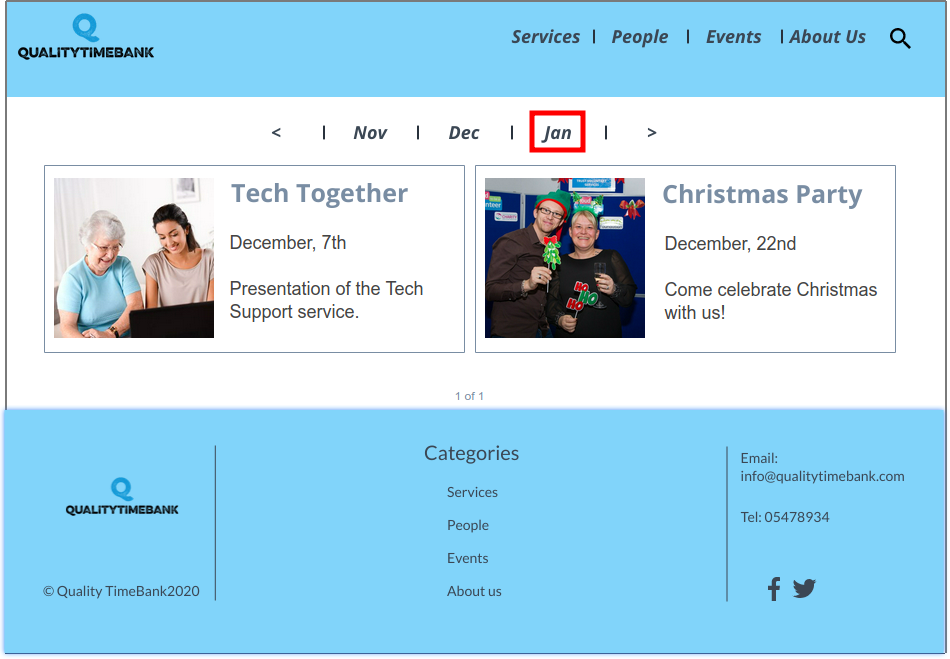
\includegraphics[width=1\linewidth, keepaspectratio]{scenarios/scenario-22}
    	\caption{}
    	\label{fig:scenario-22}
    \end{minipage}
\end{figure}

\begin{figure}[H]
    \begin{minipage}[t]{0.5\textwidth}
        \centering
    	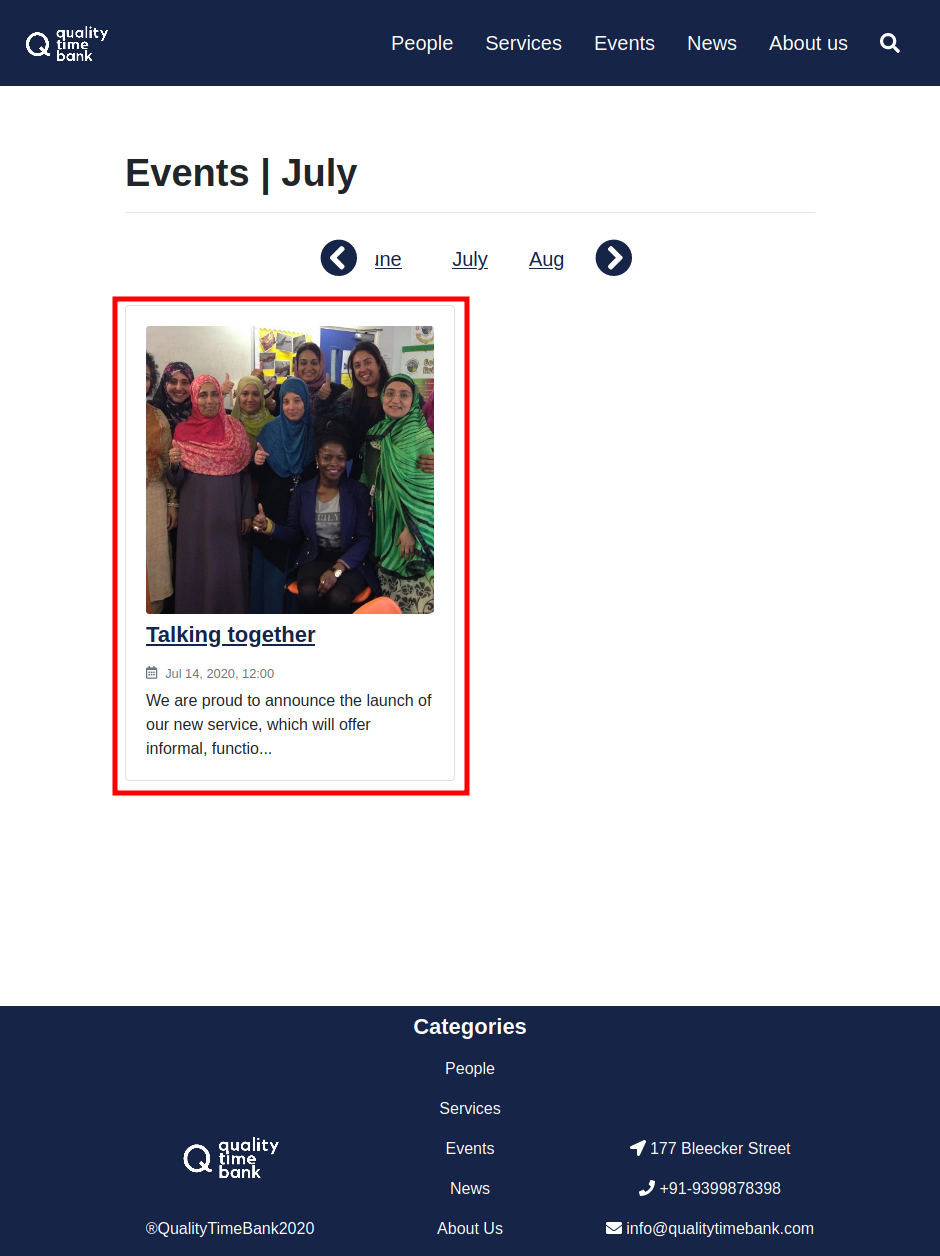
\includegraphics[width=1\linewidth, keepaspectratio]{scenarios/scenario-23}
    	\caption{}
    	\label{fig:scenario-23}
    \end{minipage}
    \hspace*{\fill}
    \begin{minipage}[t]{0.5\textwidth}
        \centering
    	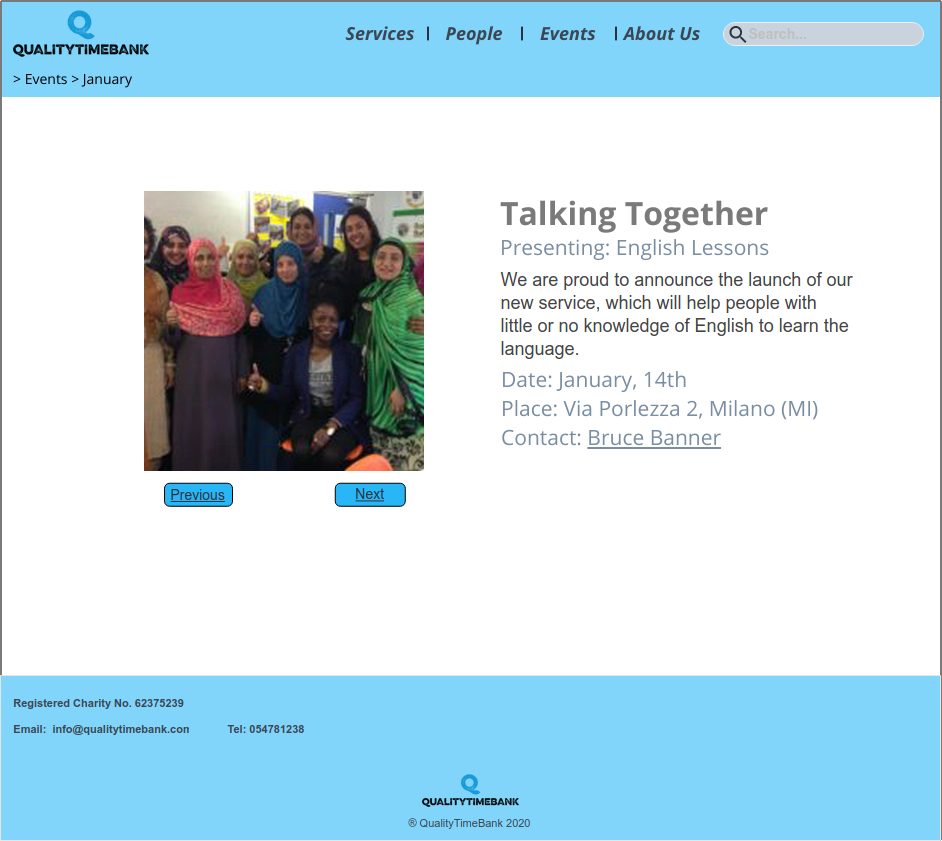
\includegraphics[width=1\linewidth, keepaspectratio]{scenarios/scenario-24}
    	\caption{}
    	\label{fig:scenario-24}
    \end{minipage}
\end{figure}

\section{Scenario 3}

The organizer of the annual Christmas party of the association has lost the phone number of the contact for the event. She clicks the "Events" button on the home page (Figure \ref{fig:scenario-31}), and she opens the event of the current month, which is December. There she reaches the page of the event (Figure \ref{fig:scenario-32}), where she can find the link of the personal page of the contact for the event (Figure \ref{fig:scenario-33}), which contains the phone number of the contact.

\begin{figure}[H]
    \begin{minipage}[t]{0.5\textwidth}
        \centering
    	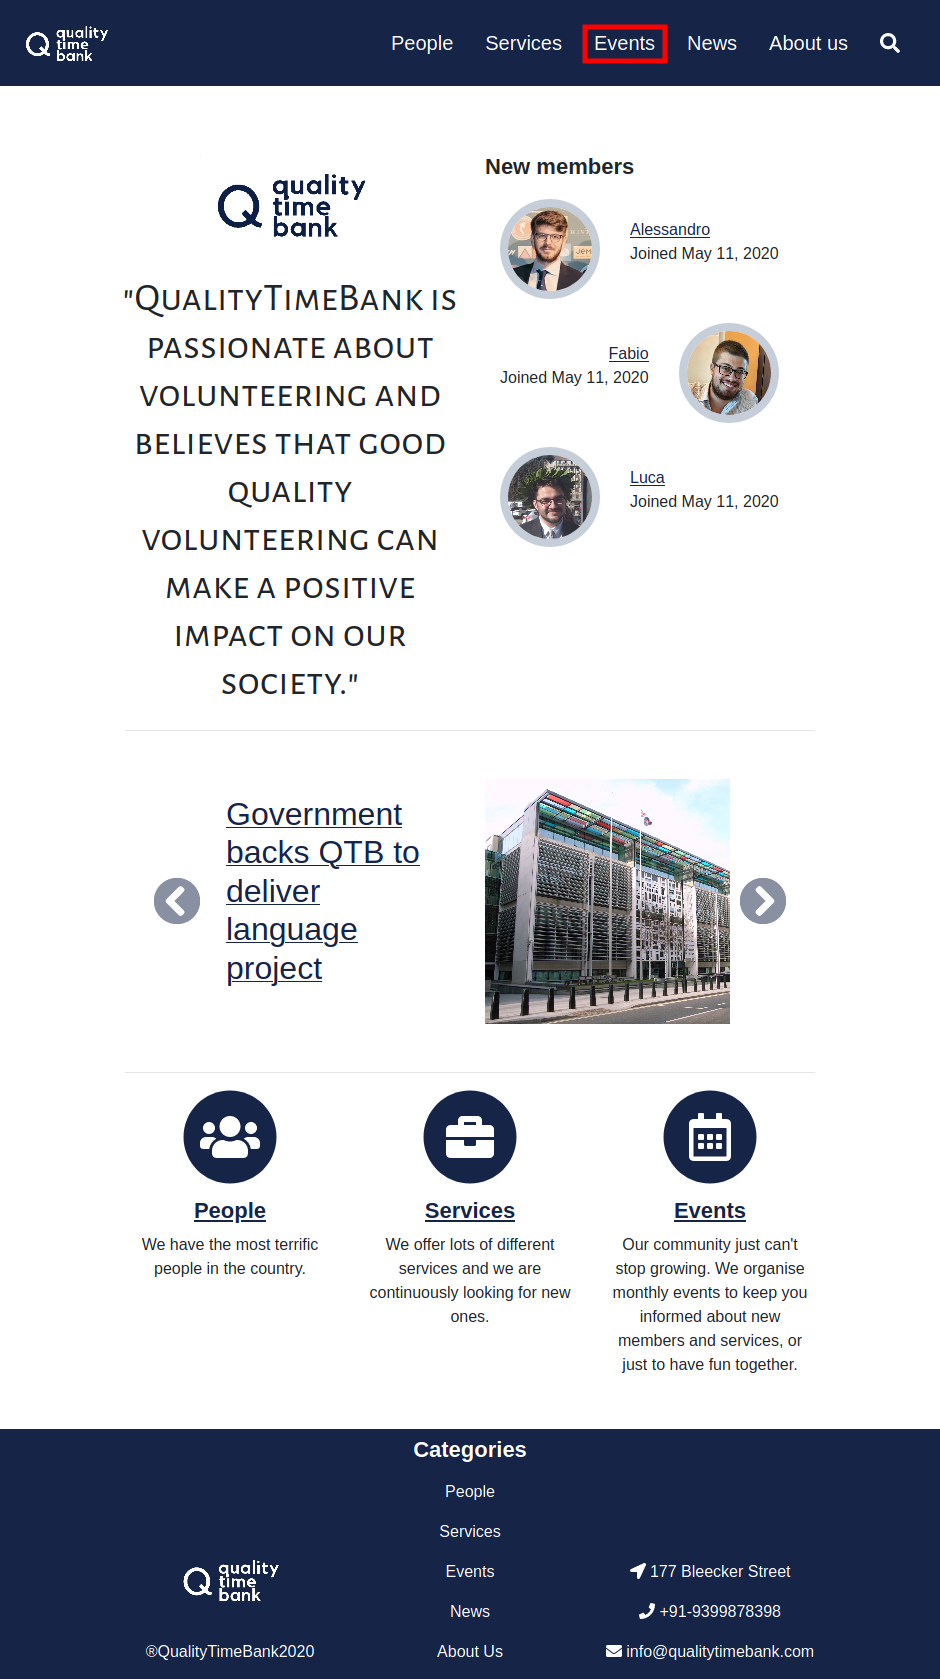
\includegraphics[width=0.9\linewidth, keepaspectratio]{scenarios/scenario-31}
    	\caption{}
    	\label{fig:scenario-31}
    \end{minipage}
    \hspace*{\fill}
    \begin{minipage}[t]{0.5\textwidth}
        \centering
    	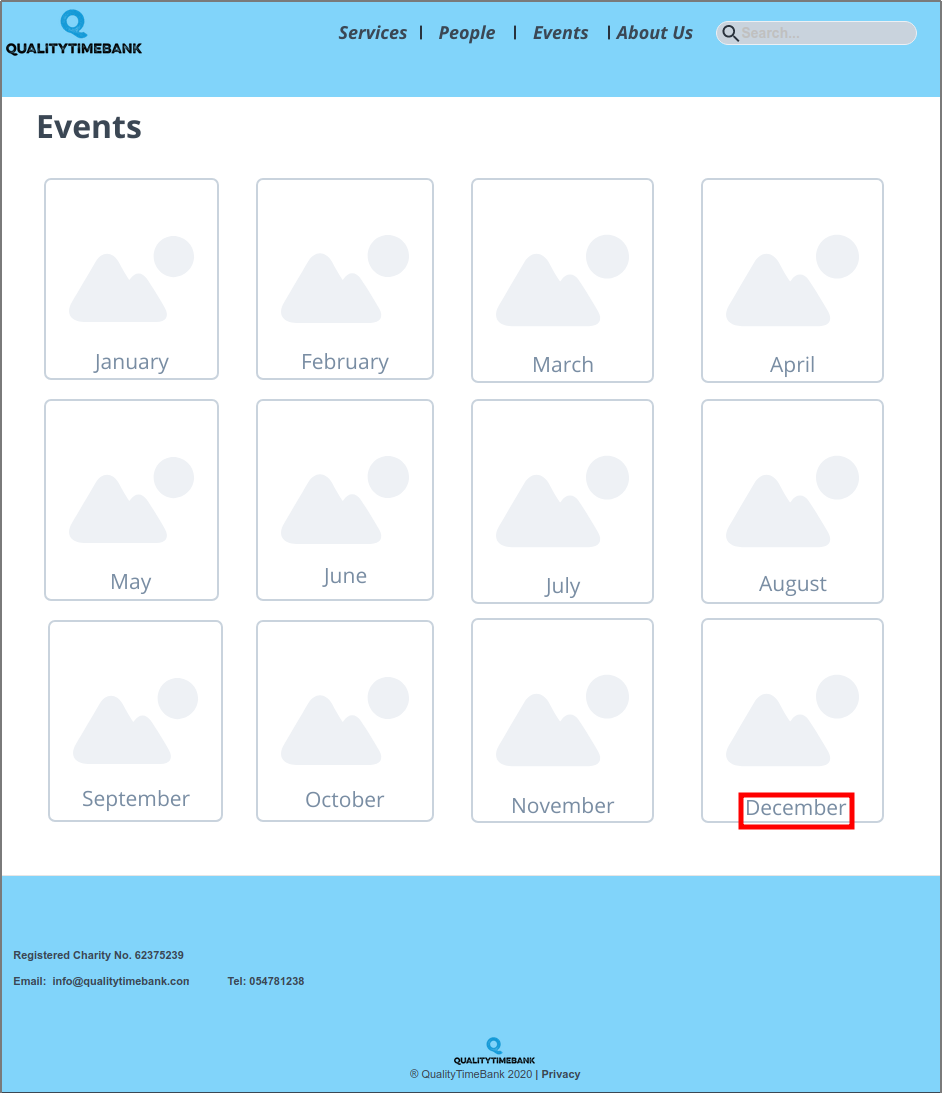
\includegraphics[width=0.9\linewidth, keepaspectratio]{scenarios/scenario-32}
    	\caption{}
    	\label{fig:scenario-32}
    \end{minipage}
\end{figure}

\begin{figure}[H]
    \centering
	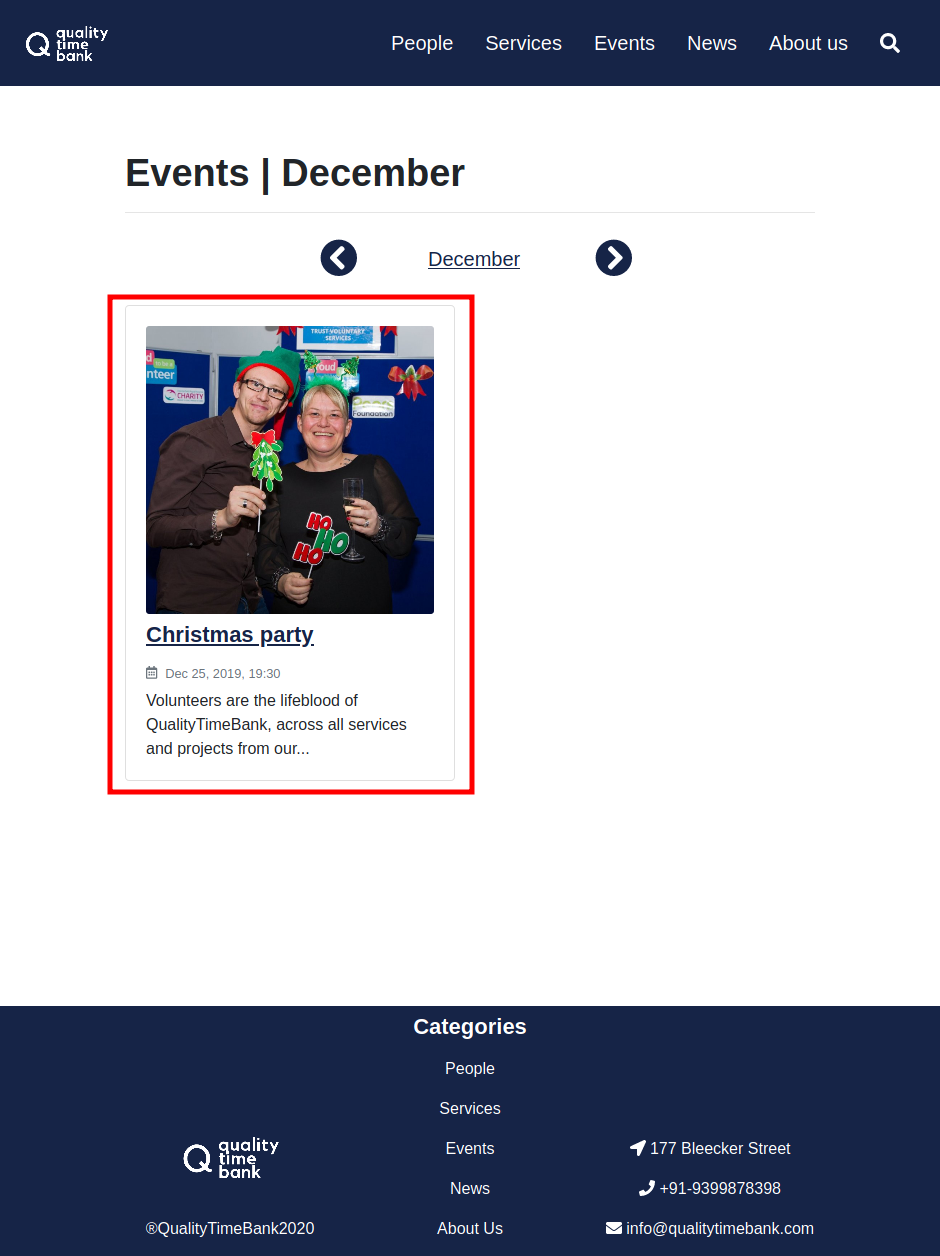
\includegraphics[width=0.4\linewidth, keepaspectratio]{scenarios/scenario-33}
	\caption{}
	\label{fig:scenario-33}
\end{figure}

\chapter{Design in the small}

\section{Home page}

\begin{figure}[H]
    \centering
    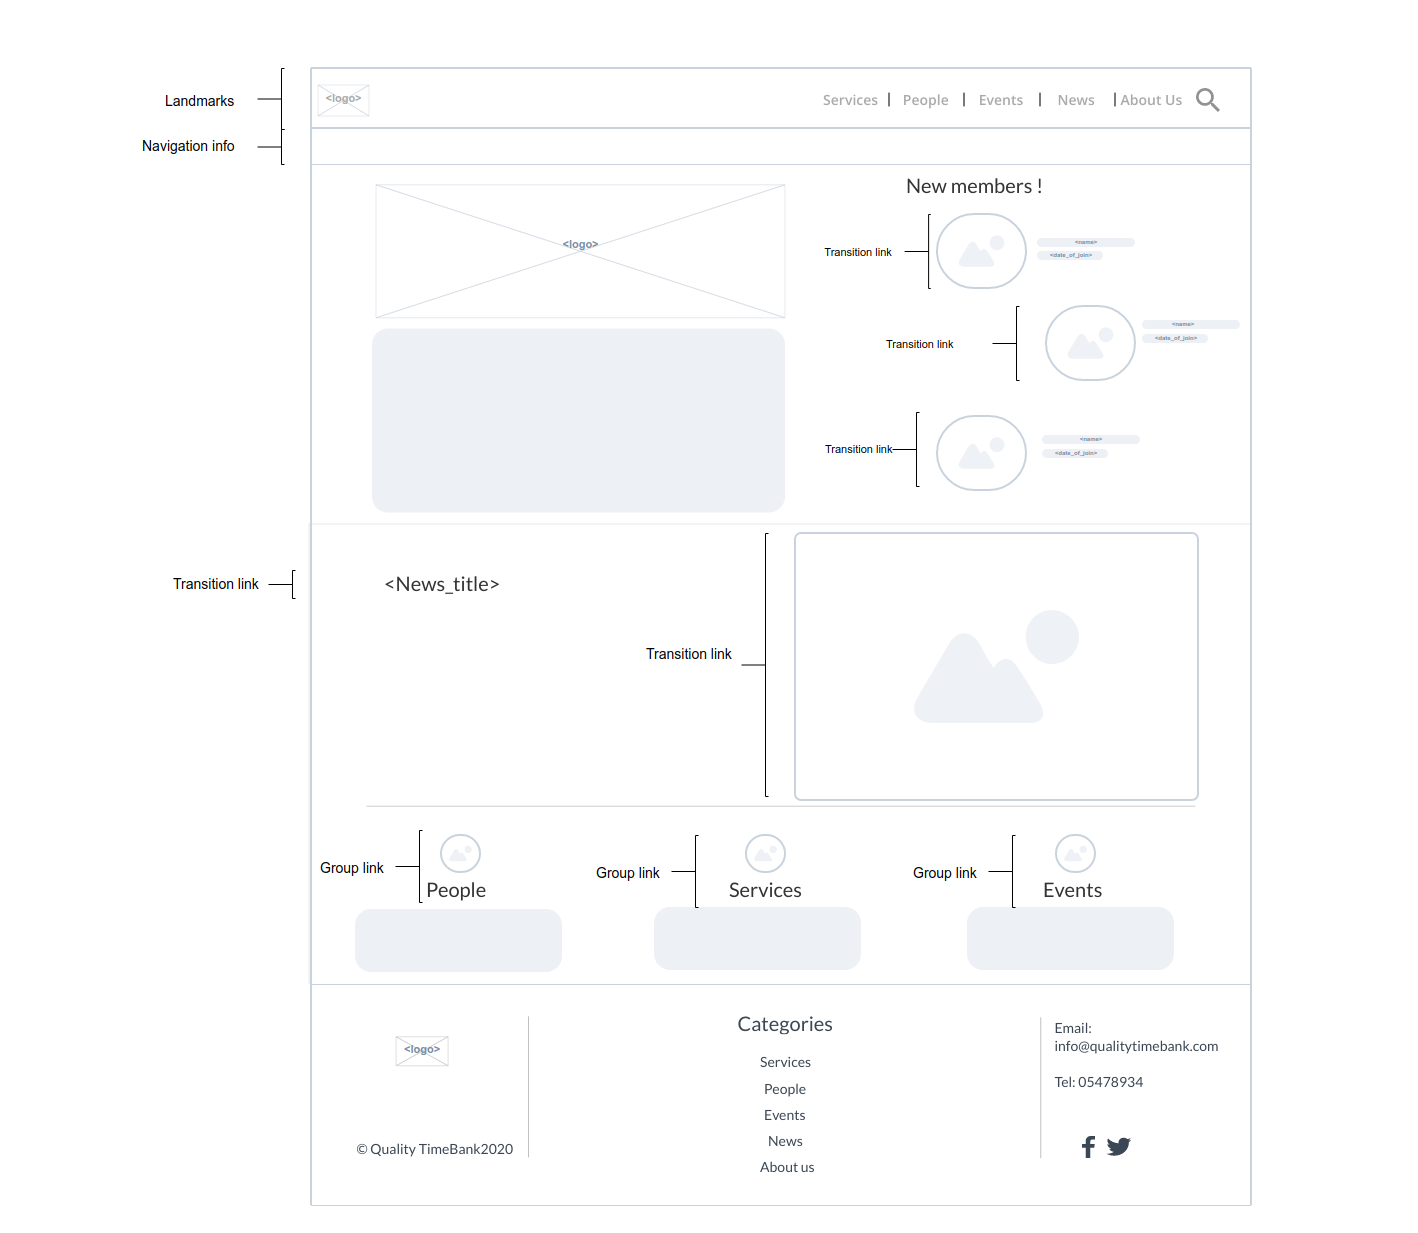
\includegraphics[width=0.93\linewidth, keepaspectratio]{wireframes/Homepage}
    \caption{Wireframe}
\end{figure}

\begin{figure}[H]
    \centering
    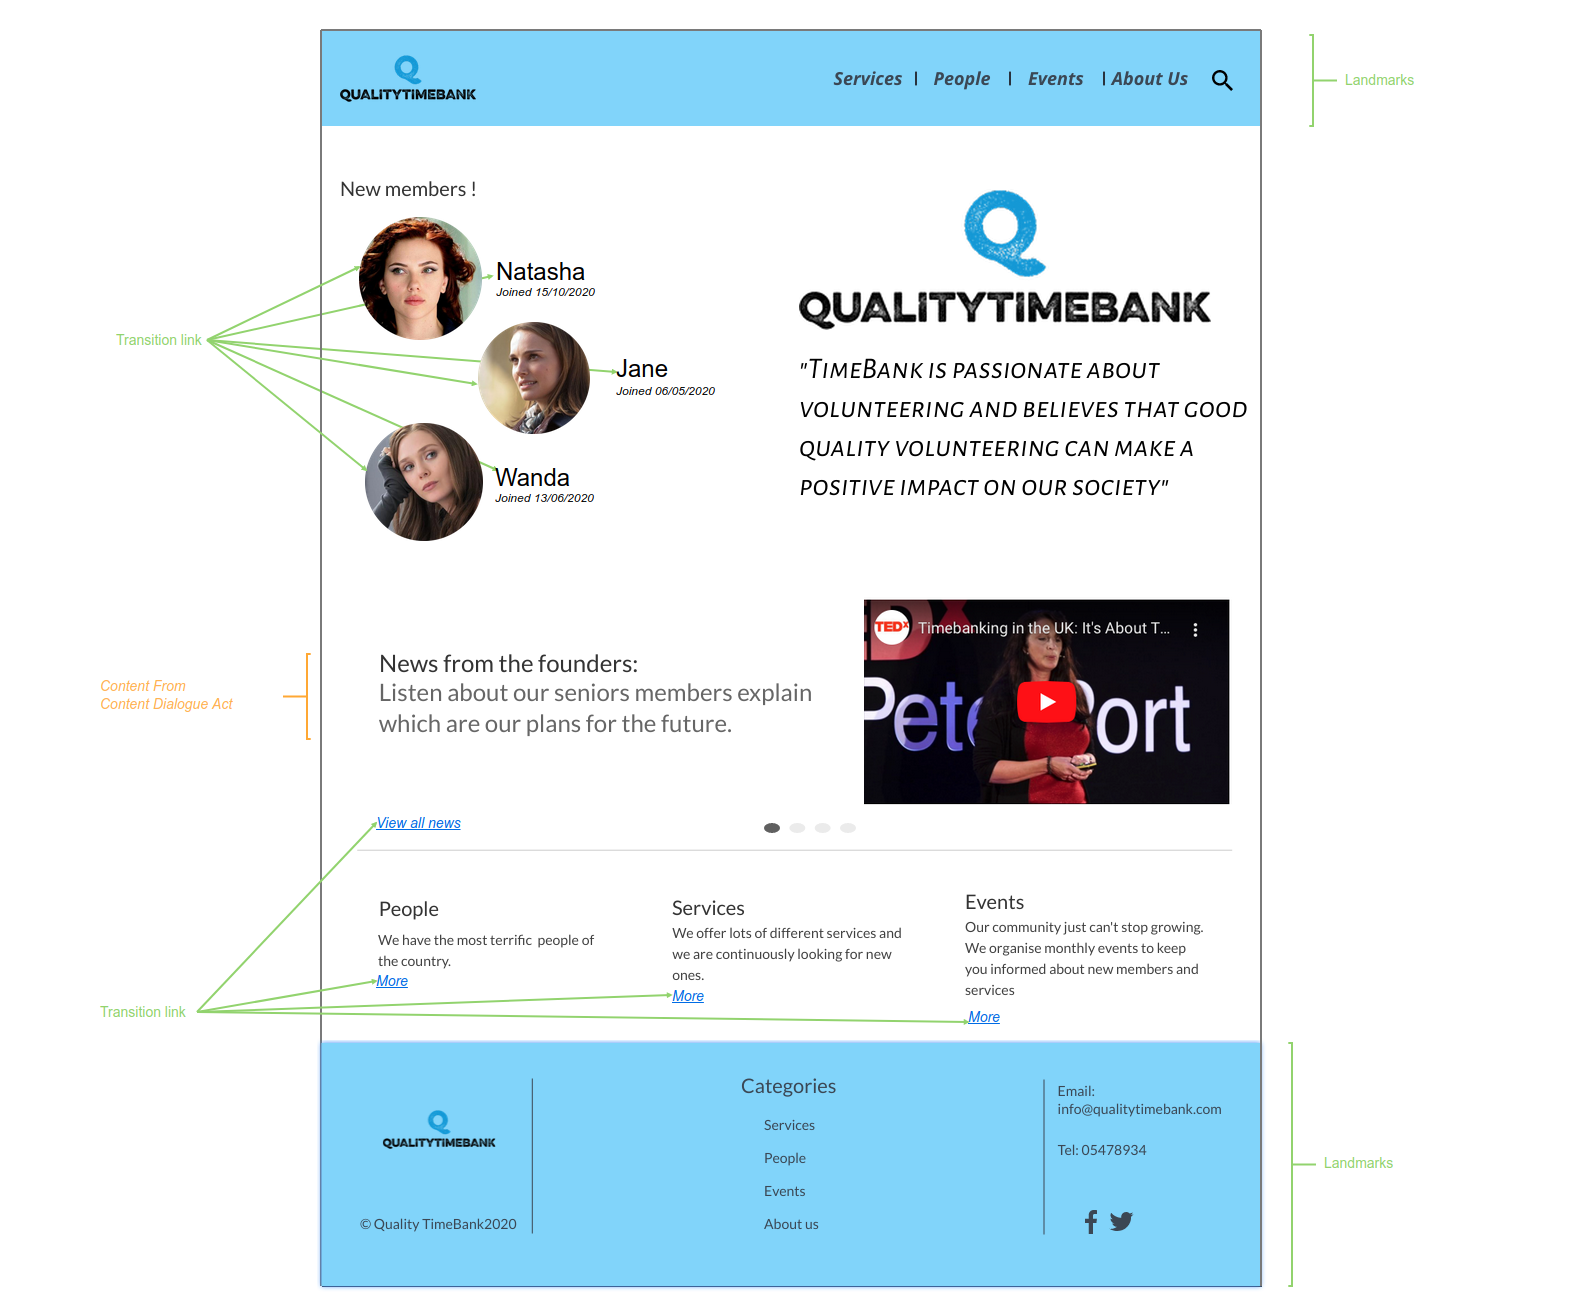
\includegraphics[width=1\linewidth, keepaspectratio]{mockups/Home_Page}
    \caption{Mockup}
\end{figure}

\section{Topic: Association}

\begin{figure}[H]
    \centering
    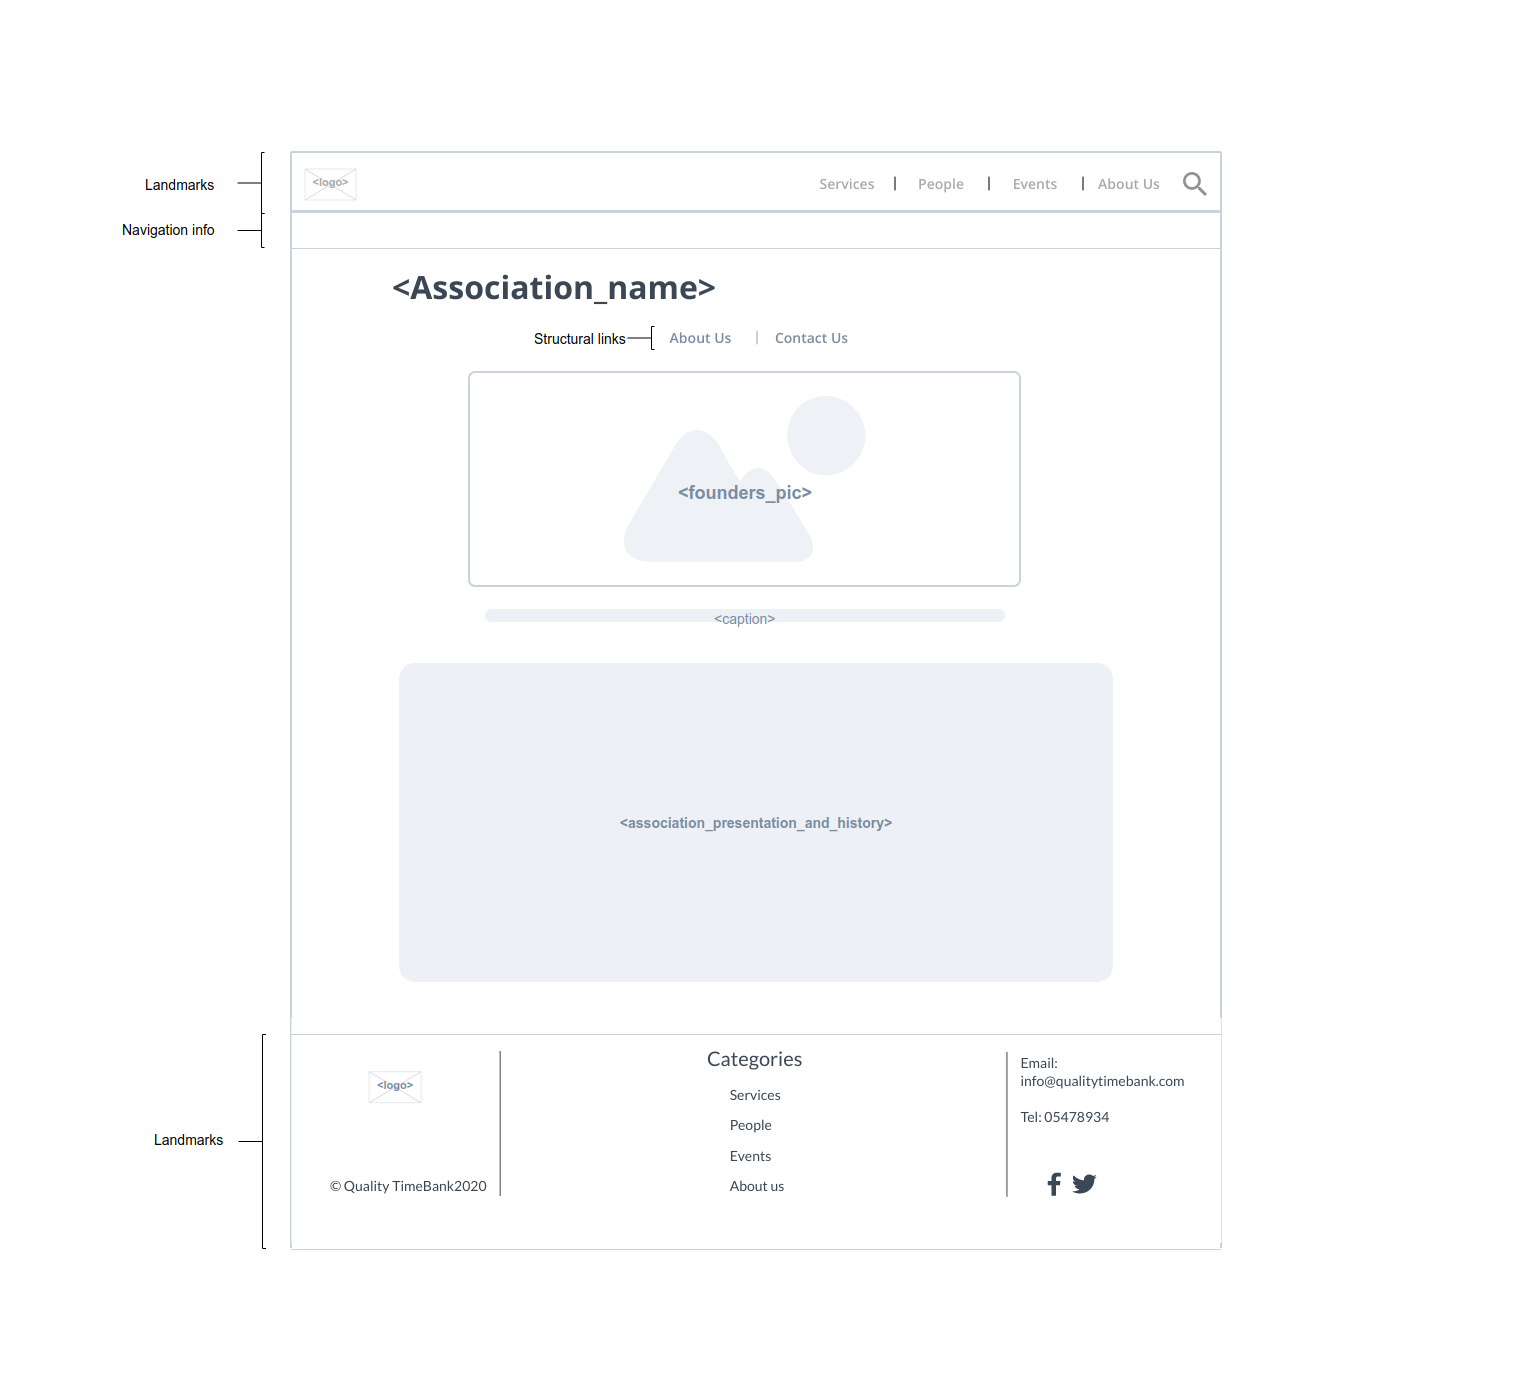
\includegraphics[width=1\linewidth, keepaspectratio]{wireframes/Topic-AboutUs}
    \caption{Wireframe}
\end{figure}

\begin{figure}[H]
    \centering
    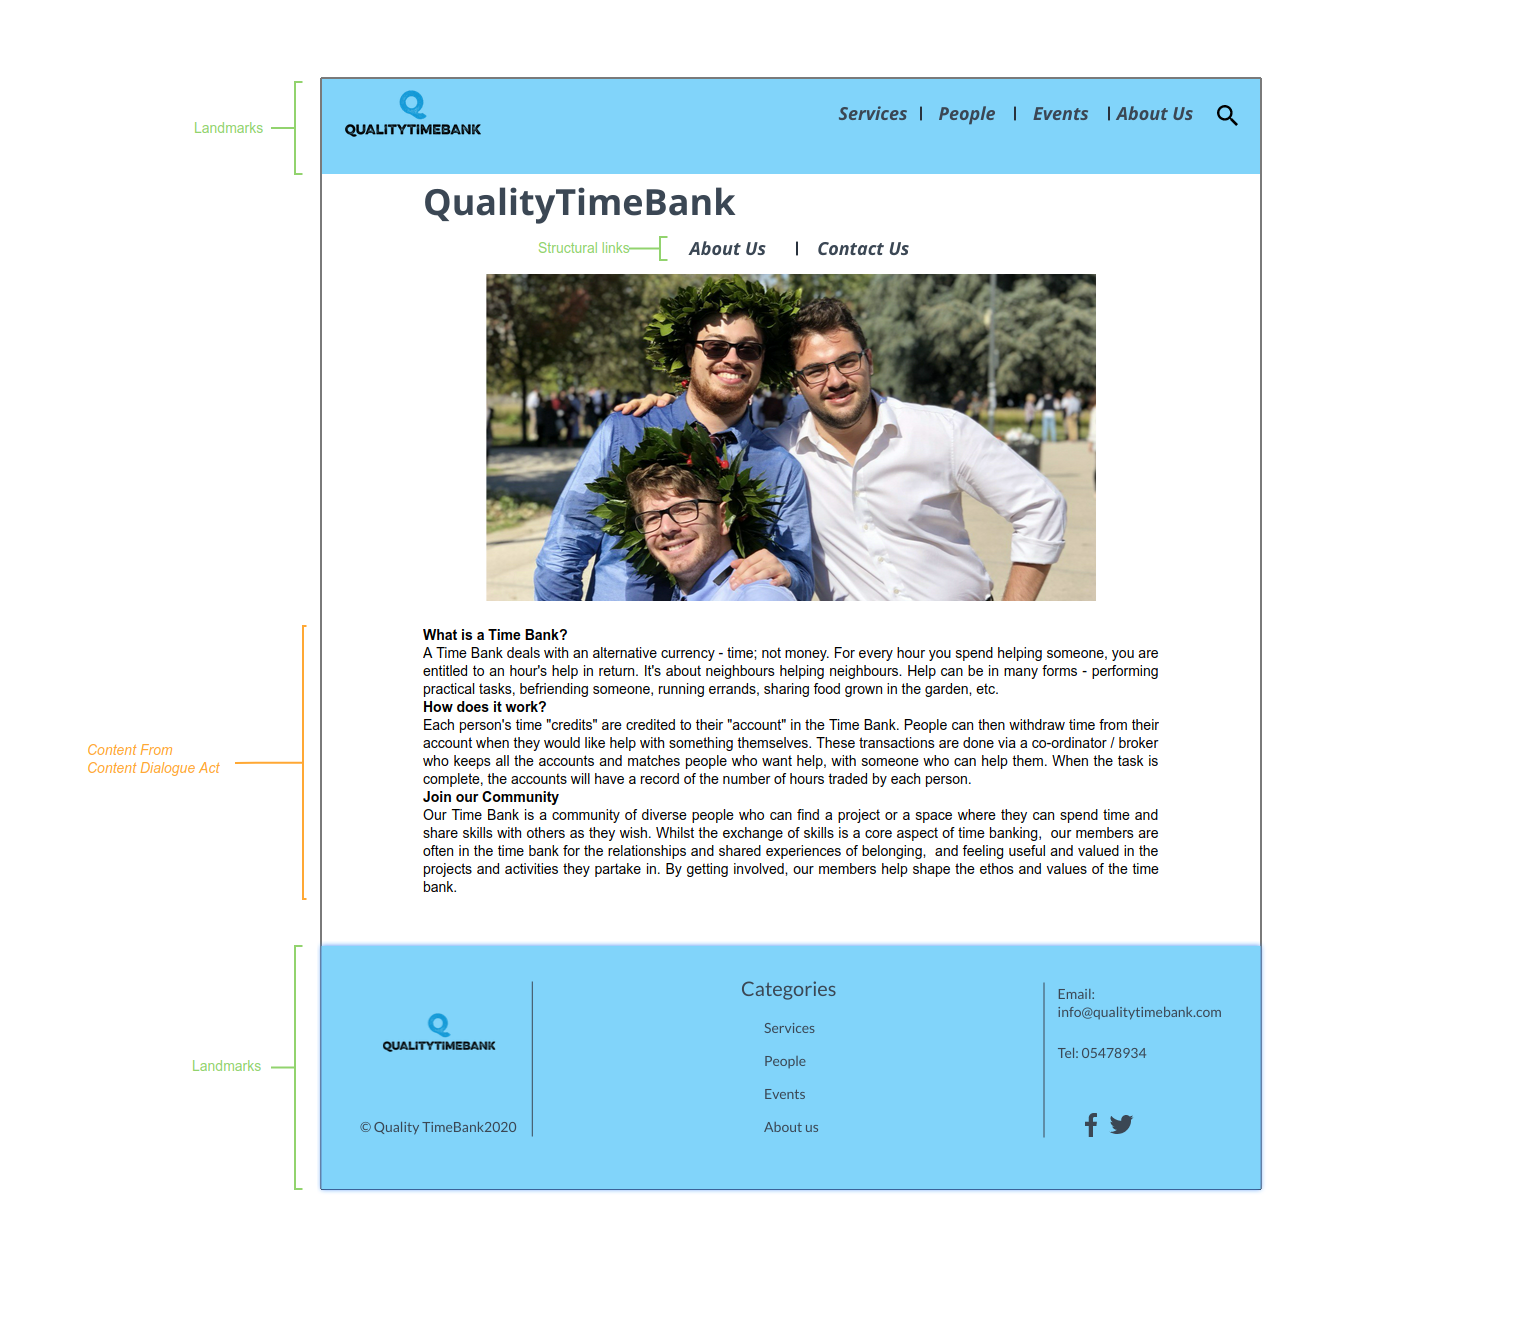
\includegraphics[width=1\linewidth, keepaspectratio]{mockups/About_Us}
    \caption{Mockup}
\end{figure}

\section{Kind of Topic: Person}

\begin{figure}[H]
    \centering
    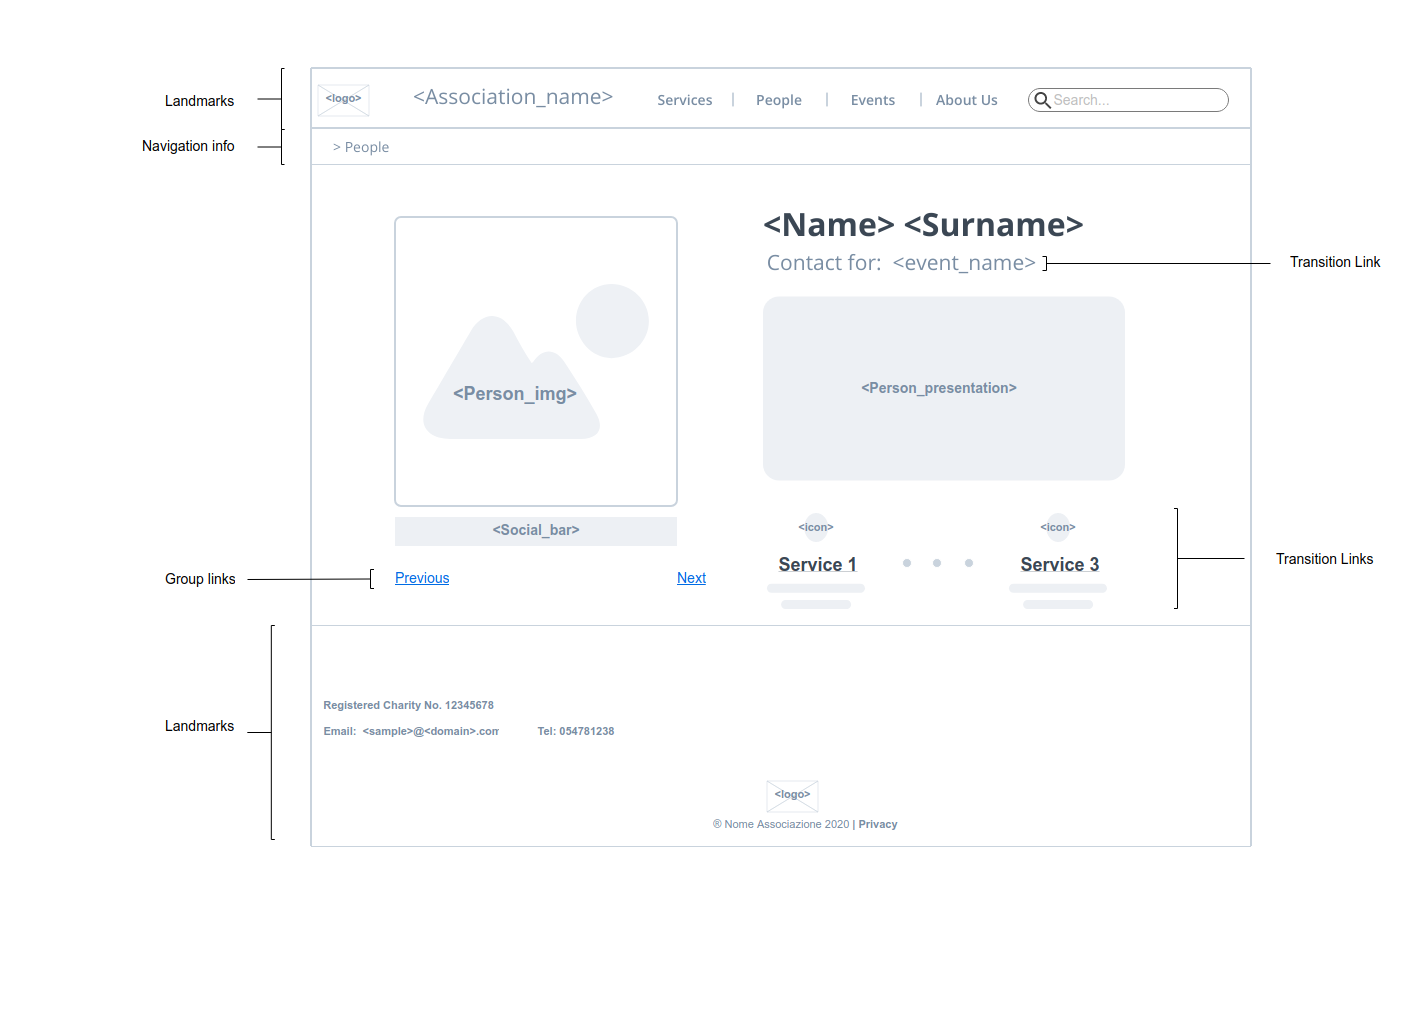
\includegraphics[width=1\linewidth, keepaspectratio]{wireframes/KindOfTopic-Person}
    \caption{Wireframe}
\end{figure}

\begin{figure}[H]
    \centering
    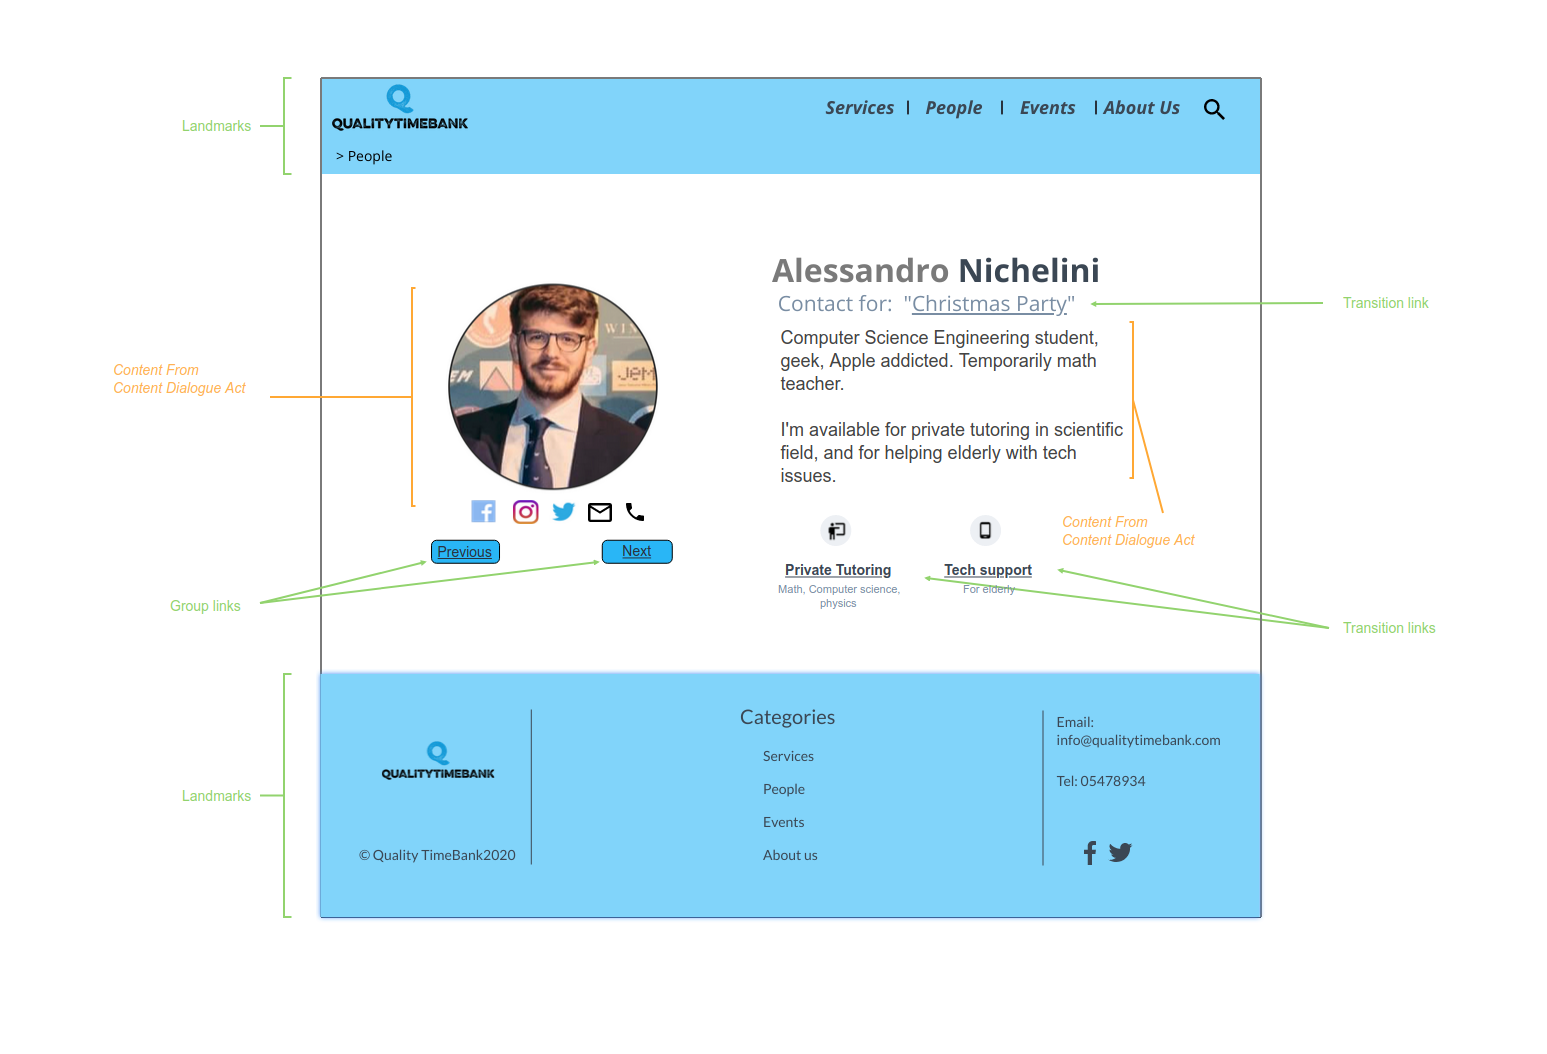
\includegraphics[width=1\linewidth, keepaspectratio]{mockups/ConcretePerson}
    \caption{Mockup}
\end{figure}

\section{Kind of Topic: Service}

\begin{figure}[H]
    \centering
    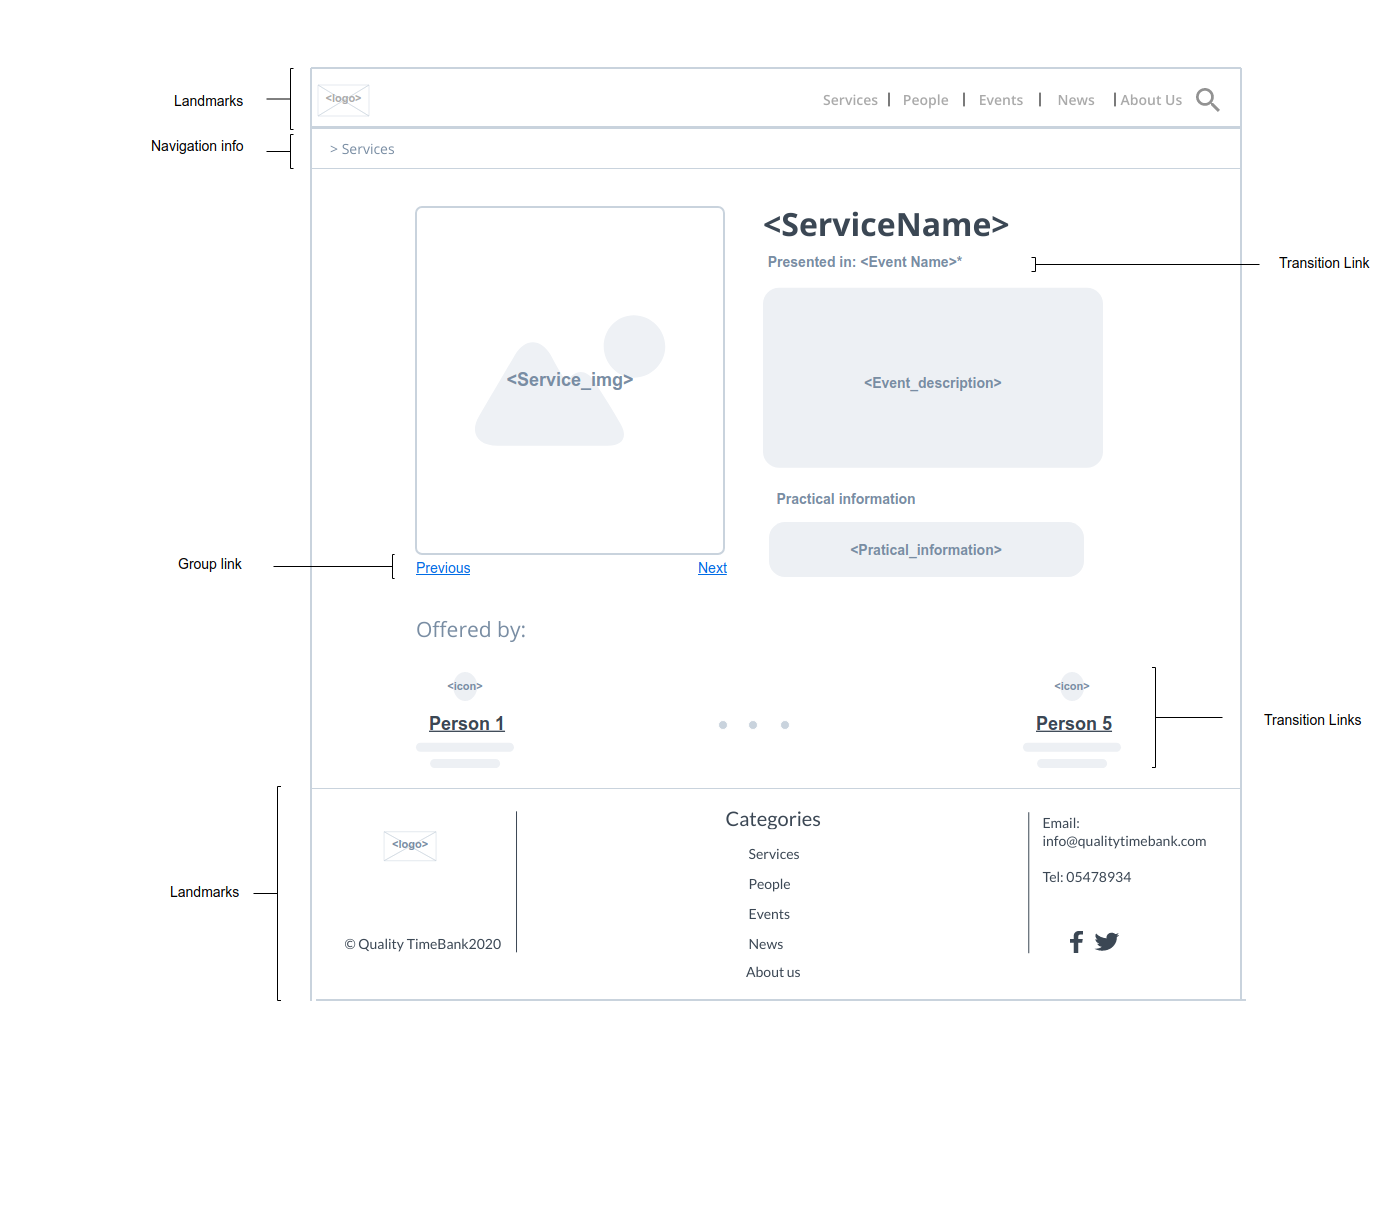
\includegraphics[width=1\linewidth, keepaspectratio]{wireframes/KindOfTopic-Service}
    \caption{Wireframe}
\end{figure}


\begin{figure}[H]
    \centering
    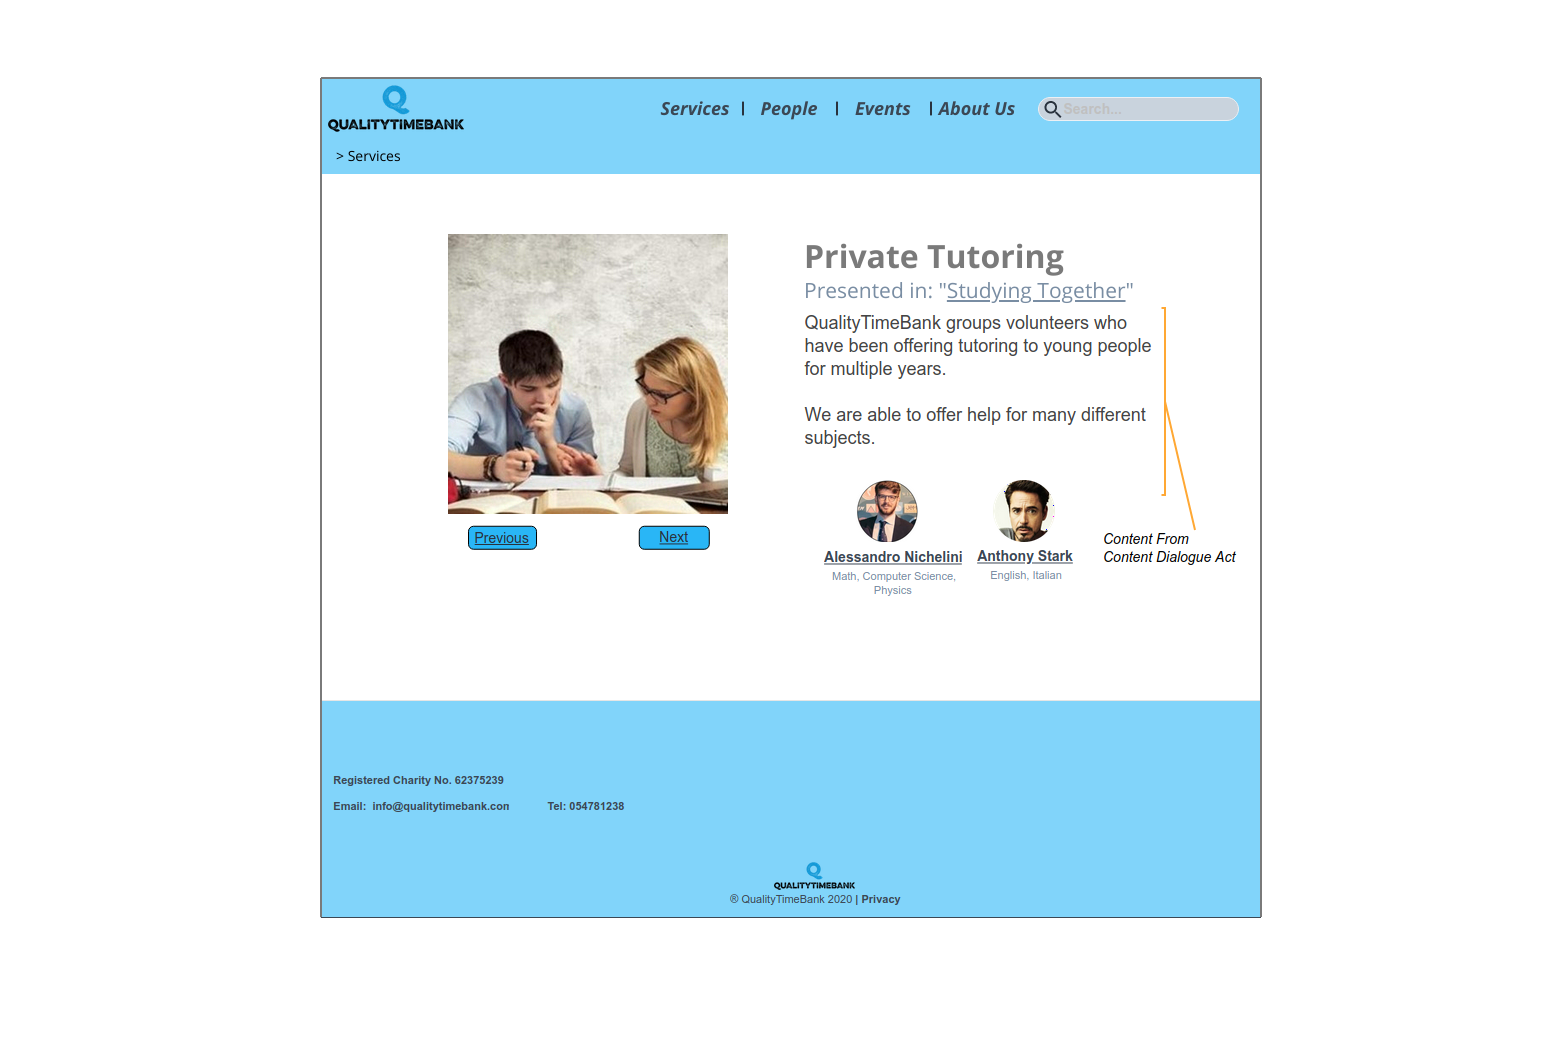
\includegraphics[width=1\linewidth, keepaspectratio]{mockups/ConcreteService}
    \caption{Mockup}
\end{figure}

\section{Kind of Topic: Event}

\begin{figure}[H]
    \centering
    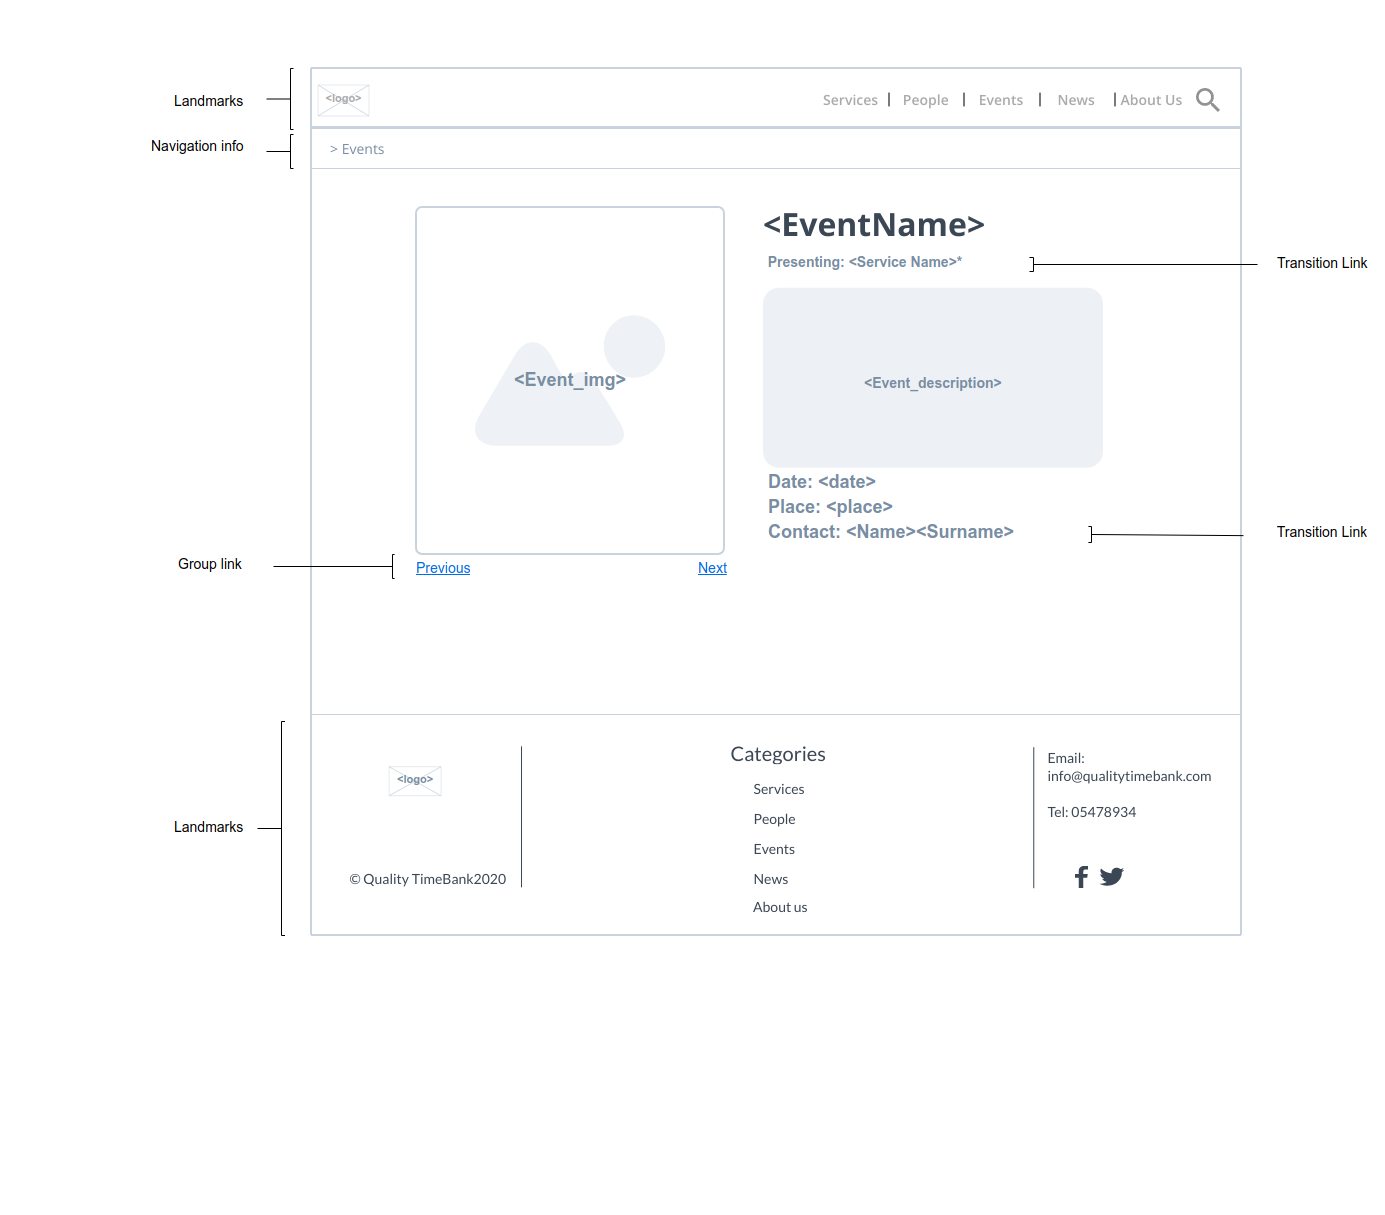
\includegraphics[width=1\linewidth, keepaspectratio]{wireframes/KindOfTopic-Event}
    \caption{Wireframe}
\end{figure}

\begin{figure}[H]
    \centering
    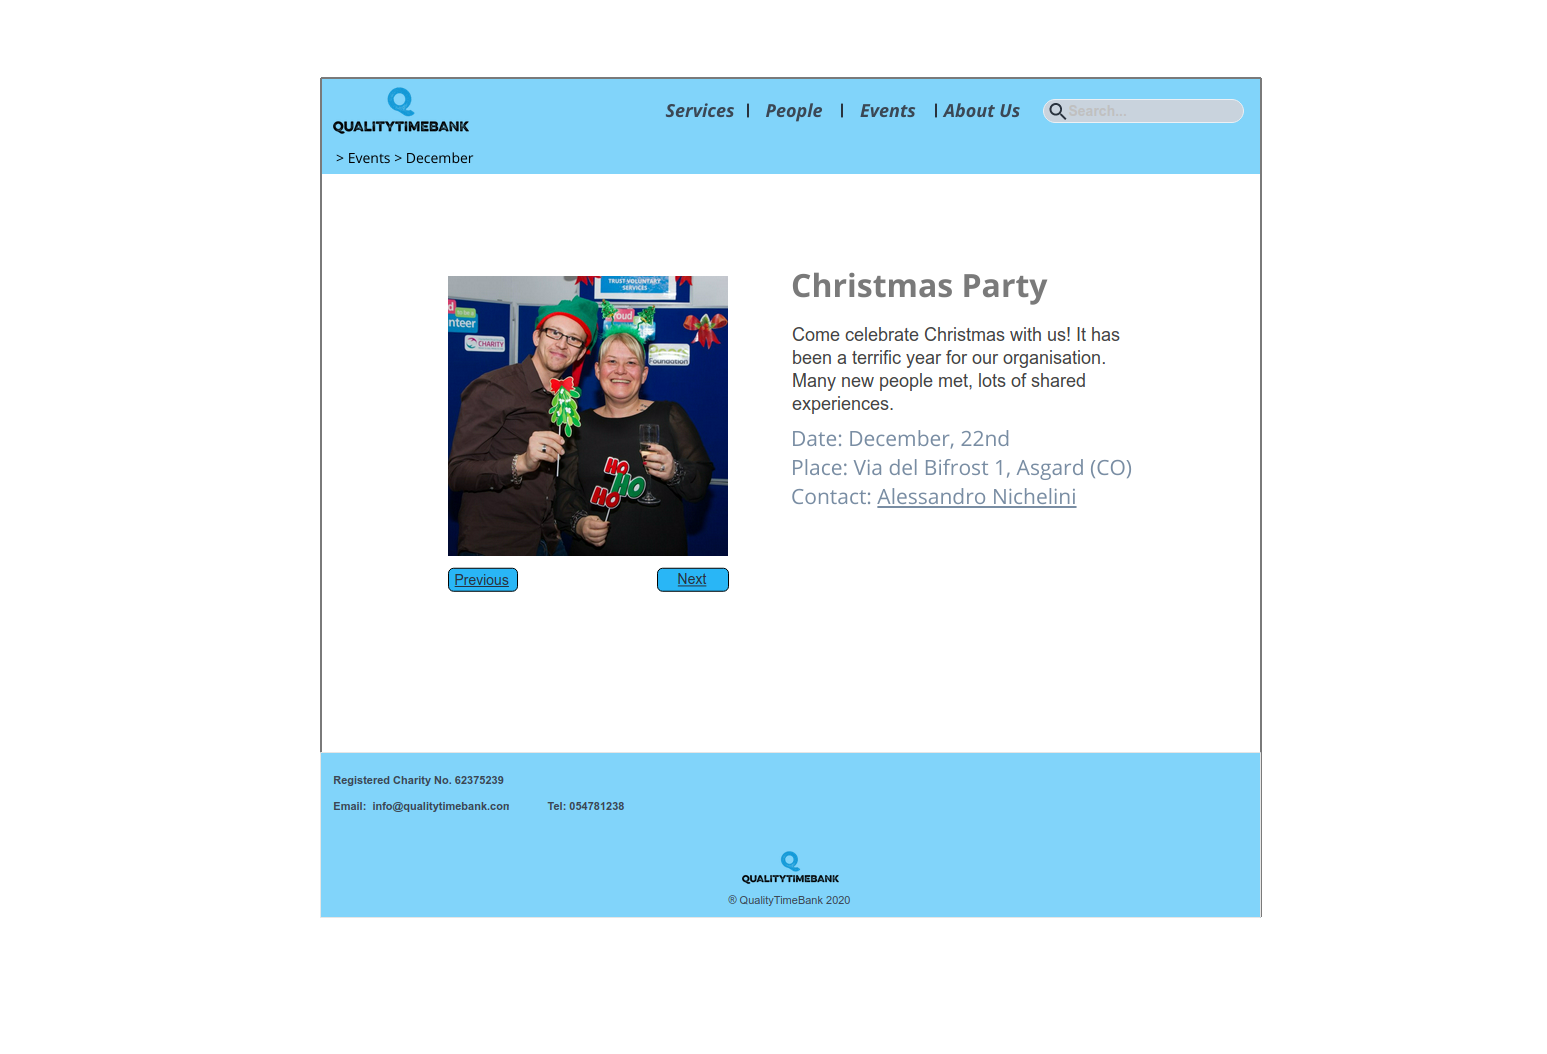
\includegraphics[width=1\linewidth, keepaspectratio]{mockups/ConcreteEventChristmas}
    \caption{Mockup}
\end{figure}

\section{Introductory page: People}

\begin{figure}[H]
    \centering
    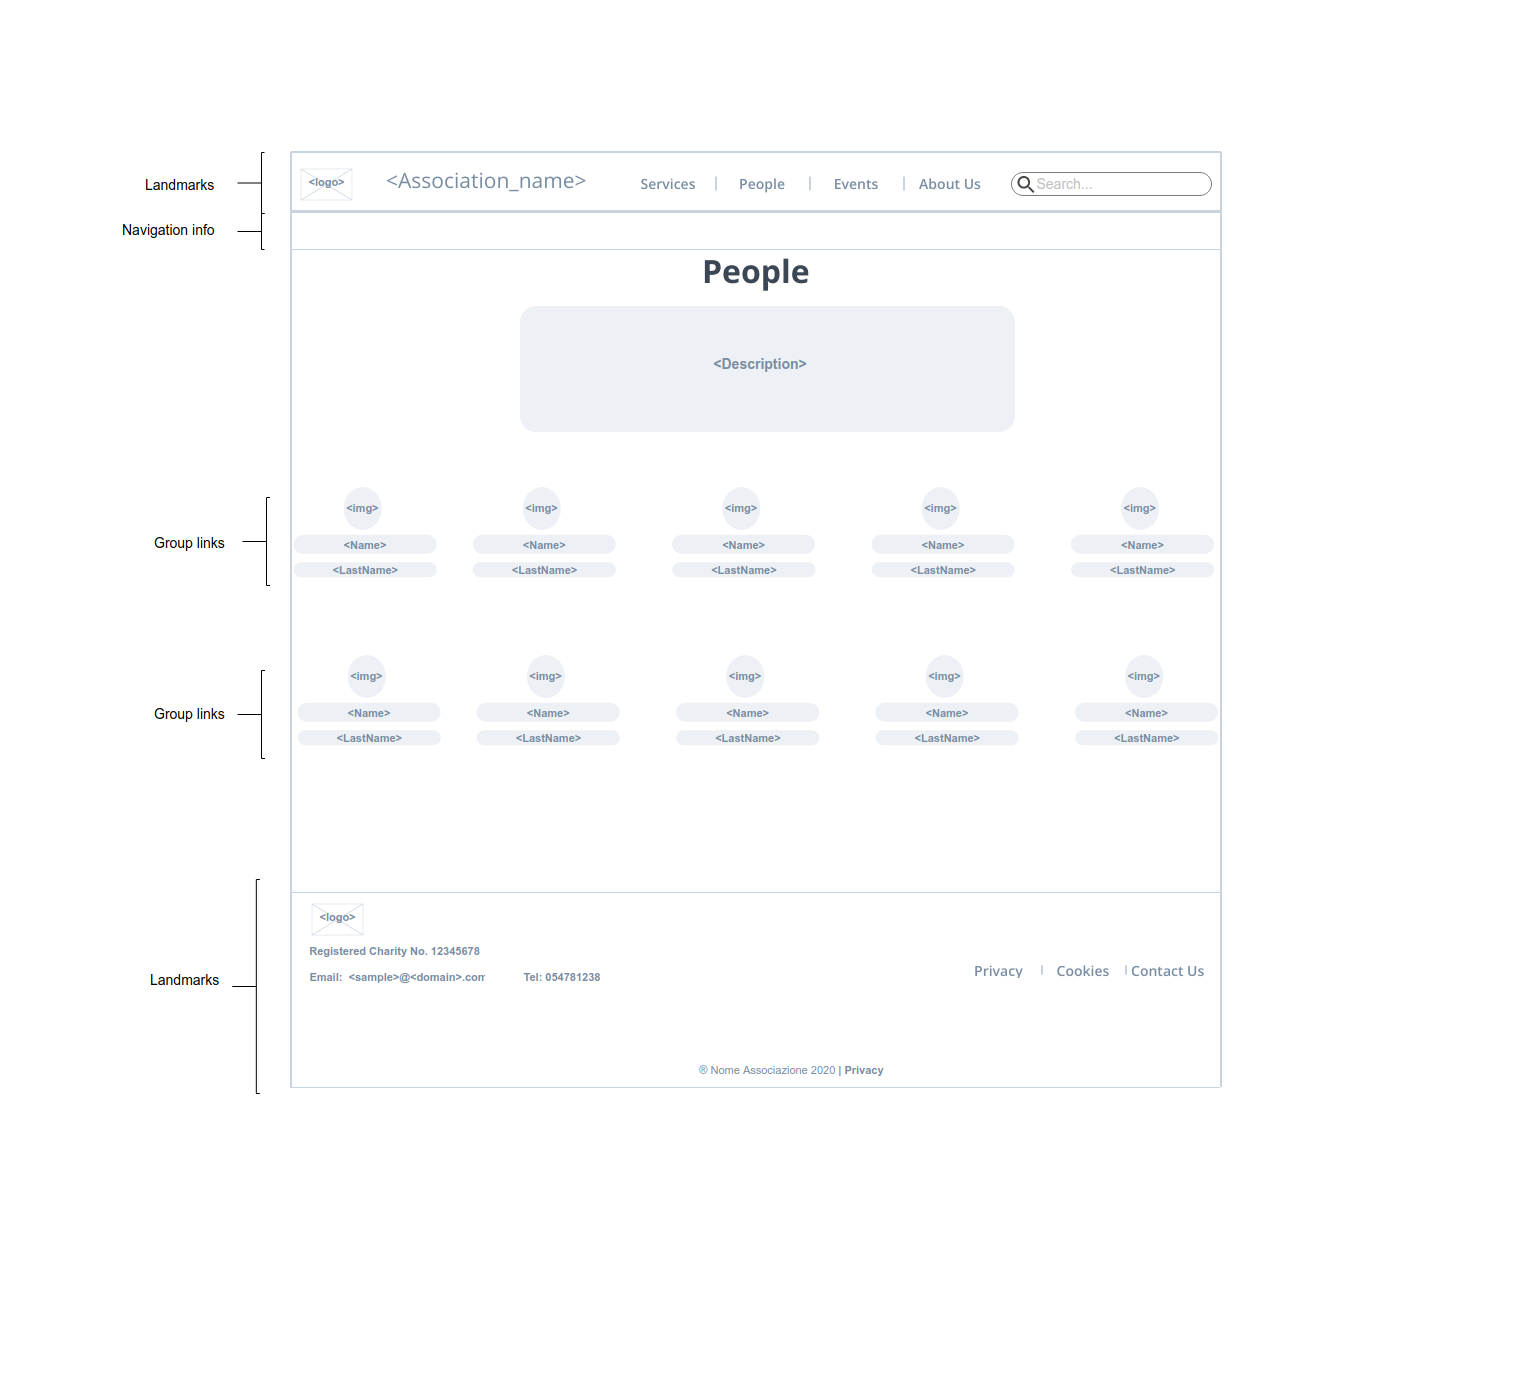
\includegraphics[width=1\linewidth, keepaspectratio]{wireframes/Introductory-People}
    \caption{Wireframe}
\end{figure}

\begin{figure}[H]
    \centering
    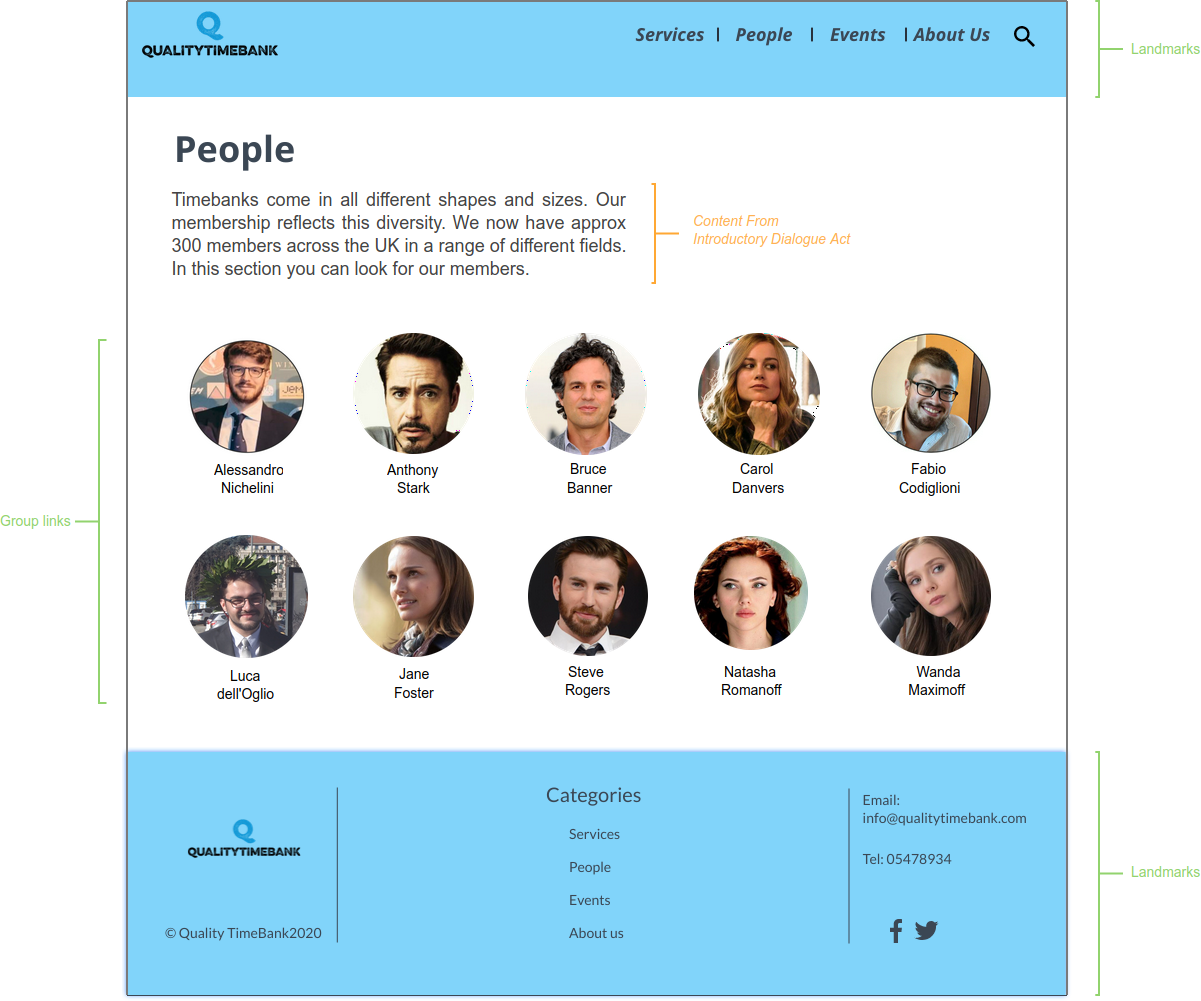
\includegraphics[width=1\linewidth, keepaspectratio]{mockups/ConcretePeople}
    \caption{Mockup}
\end{figure}

\section{Introductory page: Services}

\begin{figure}[H]
    \centering
    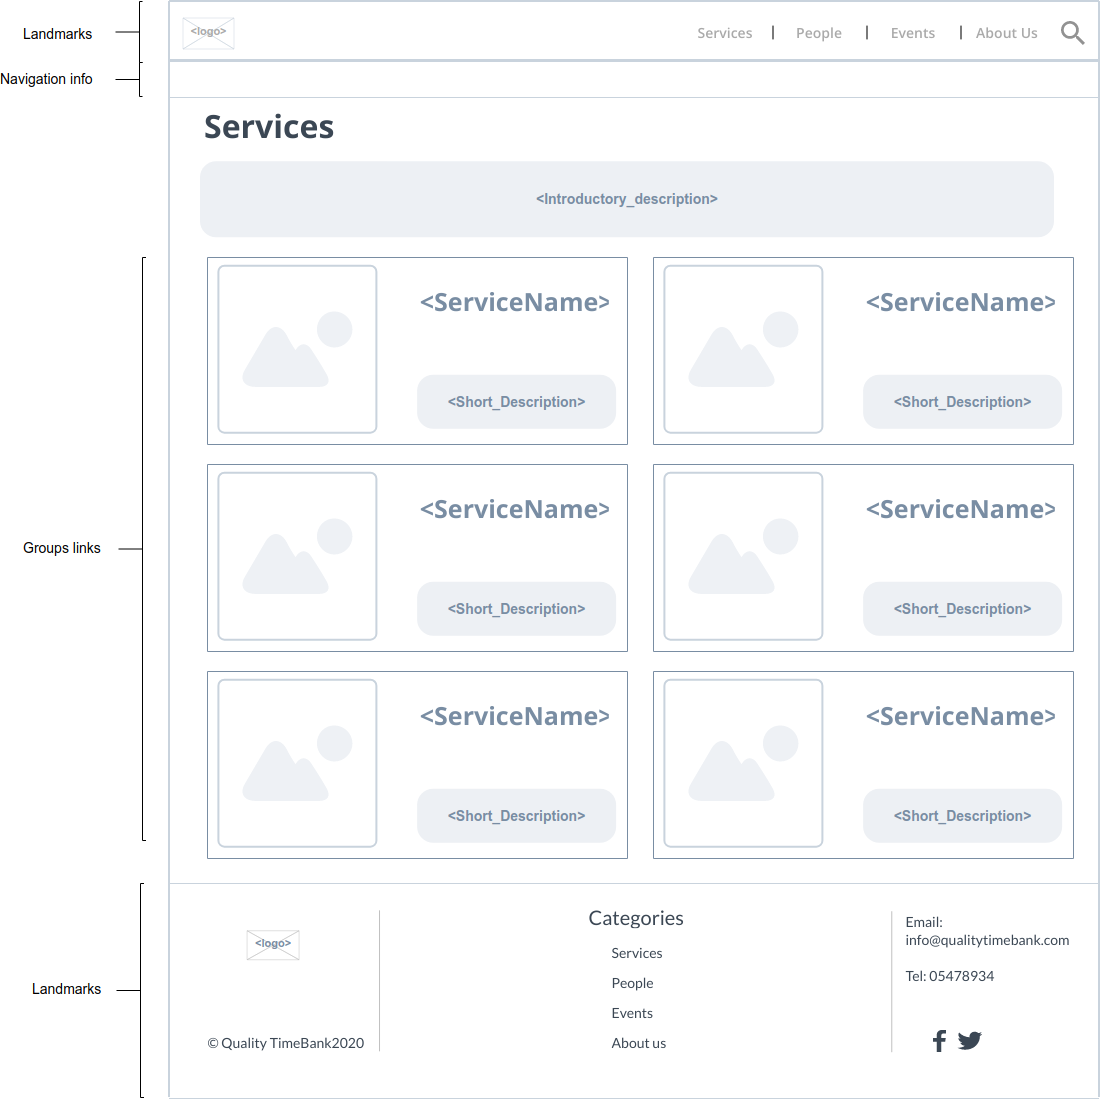
\includegraphics[width=1\linewidth, keepaspectratio]{wireframes/Introductory-Services}
    \caption{Wireframe}
\end{figure}

\begin{figure}[H]
    \centering
    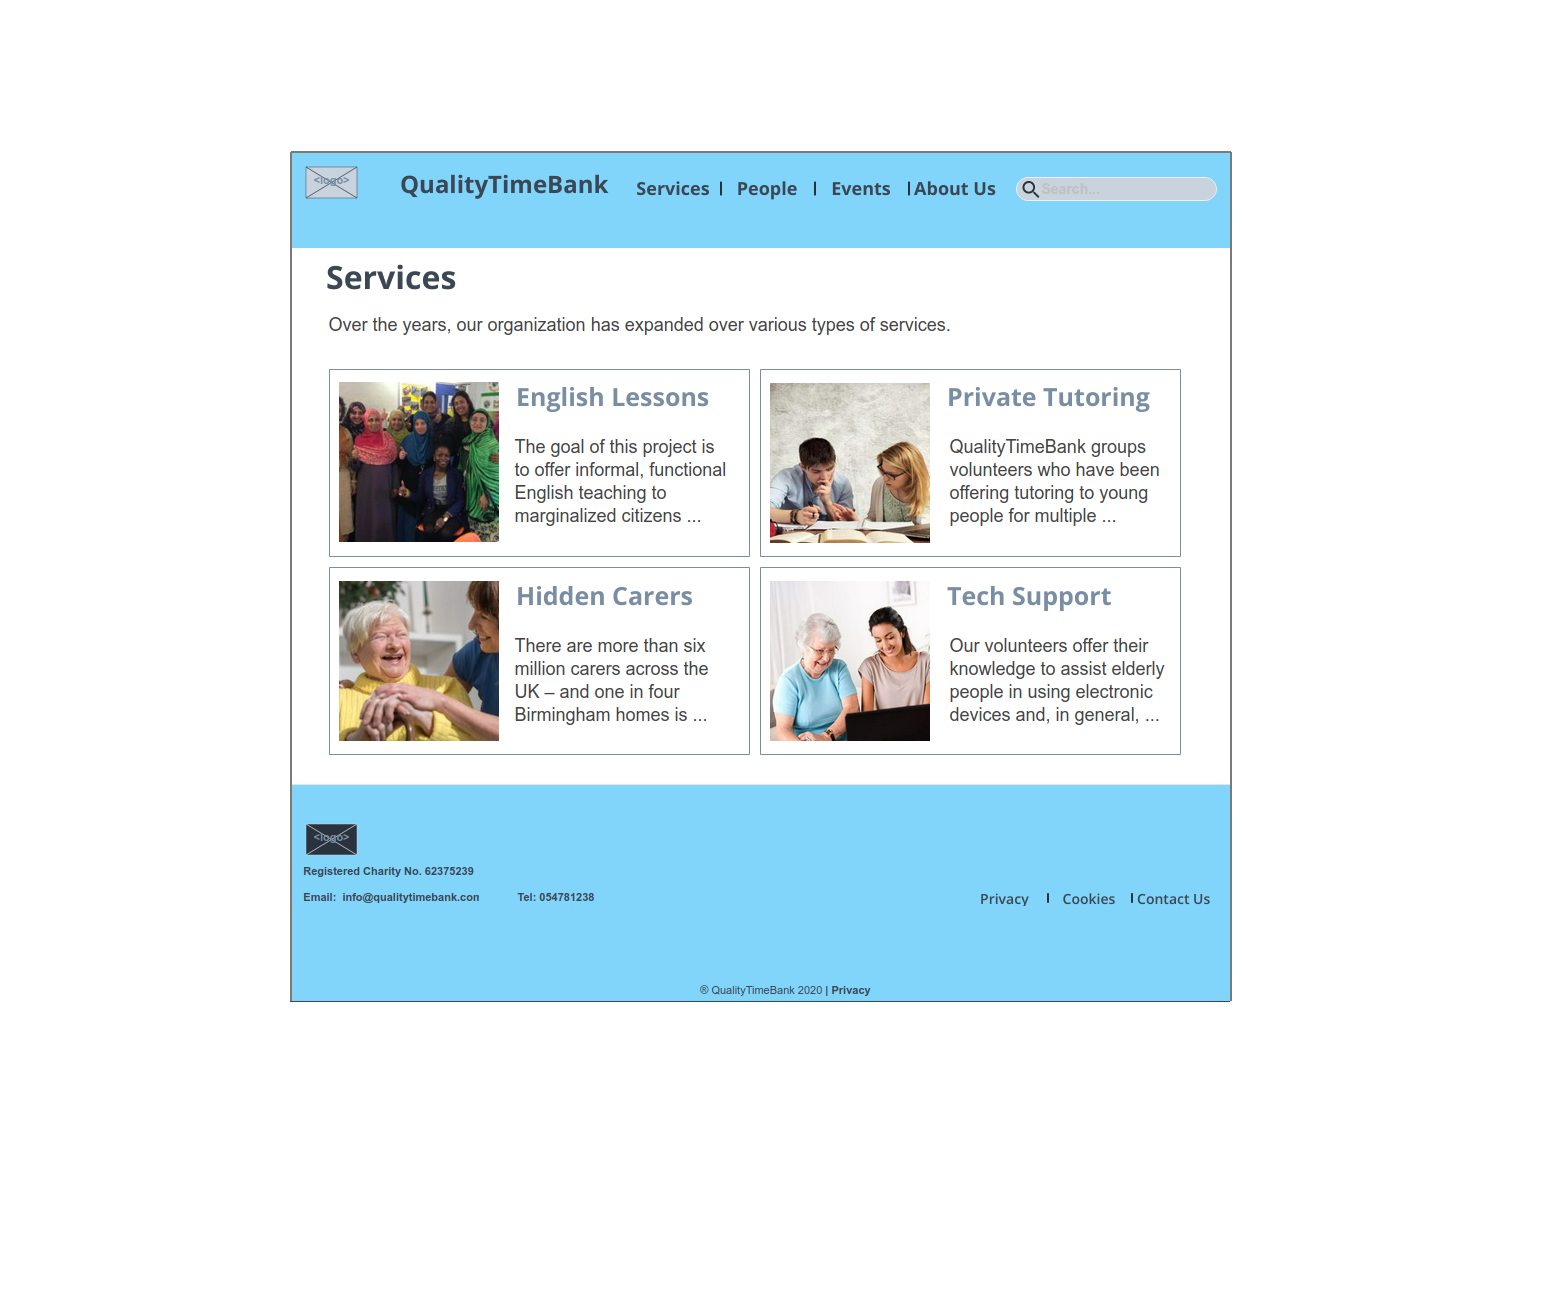
\includegraphics[width=1\linewidth, keepaspectratio]{mockups/ConcreteServices}
    \caption{Mockup}
\end{figure}

\section{Introductory page: Events}

\begin{figure}[H]
    \centering
    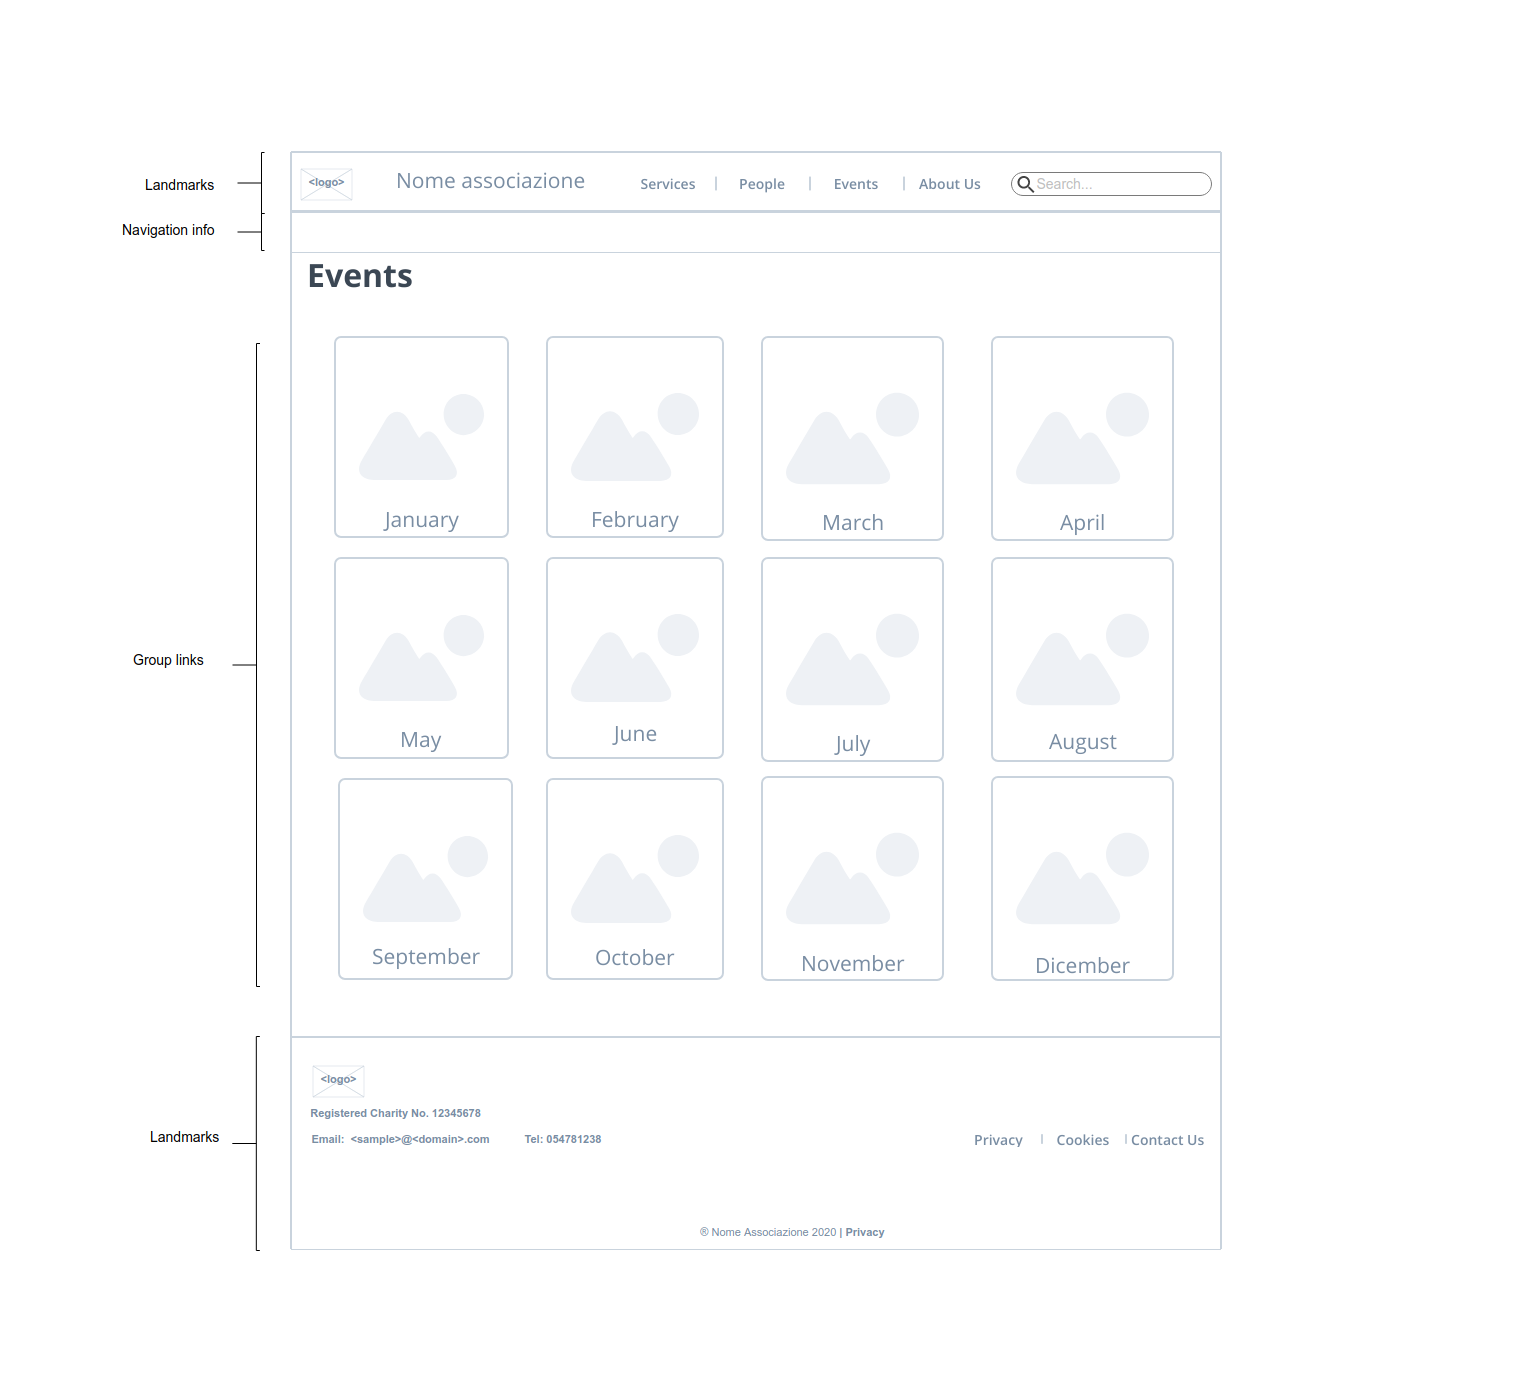
\includegraphics[width=1\linewidth, keepaspectratio]{wireframes/Introductory-Events}
    \caption{Wireframe}
\end{figure}

\begin{figure}[H]
    \centering
    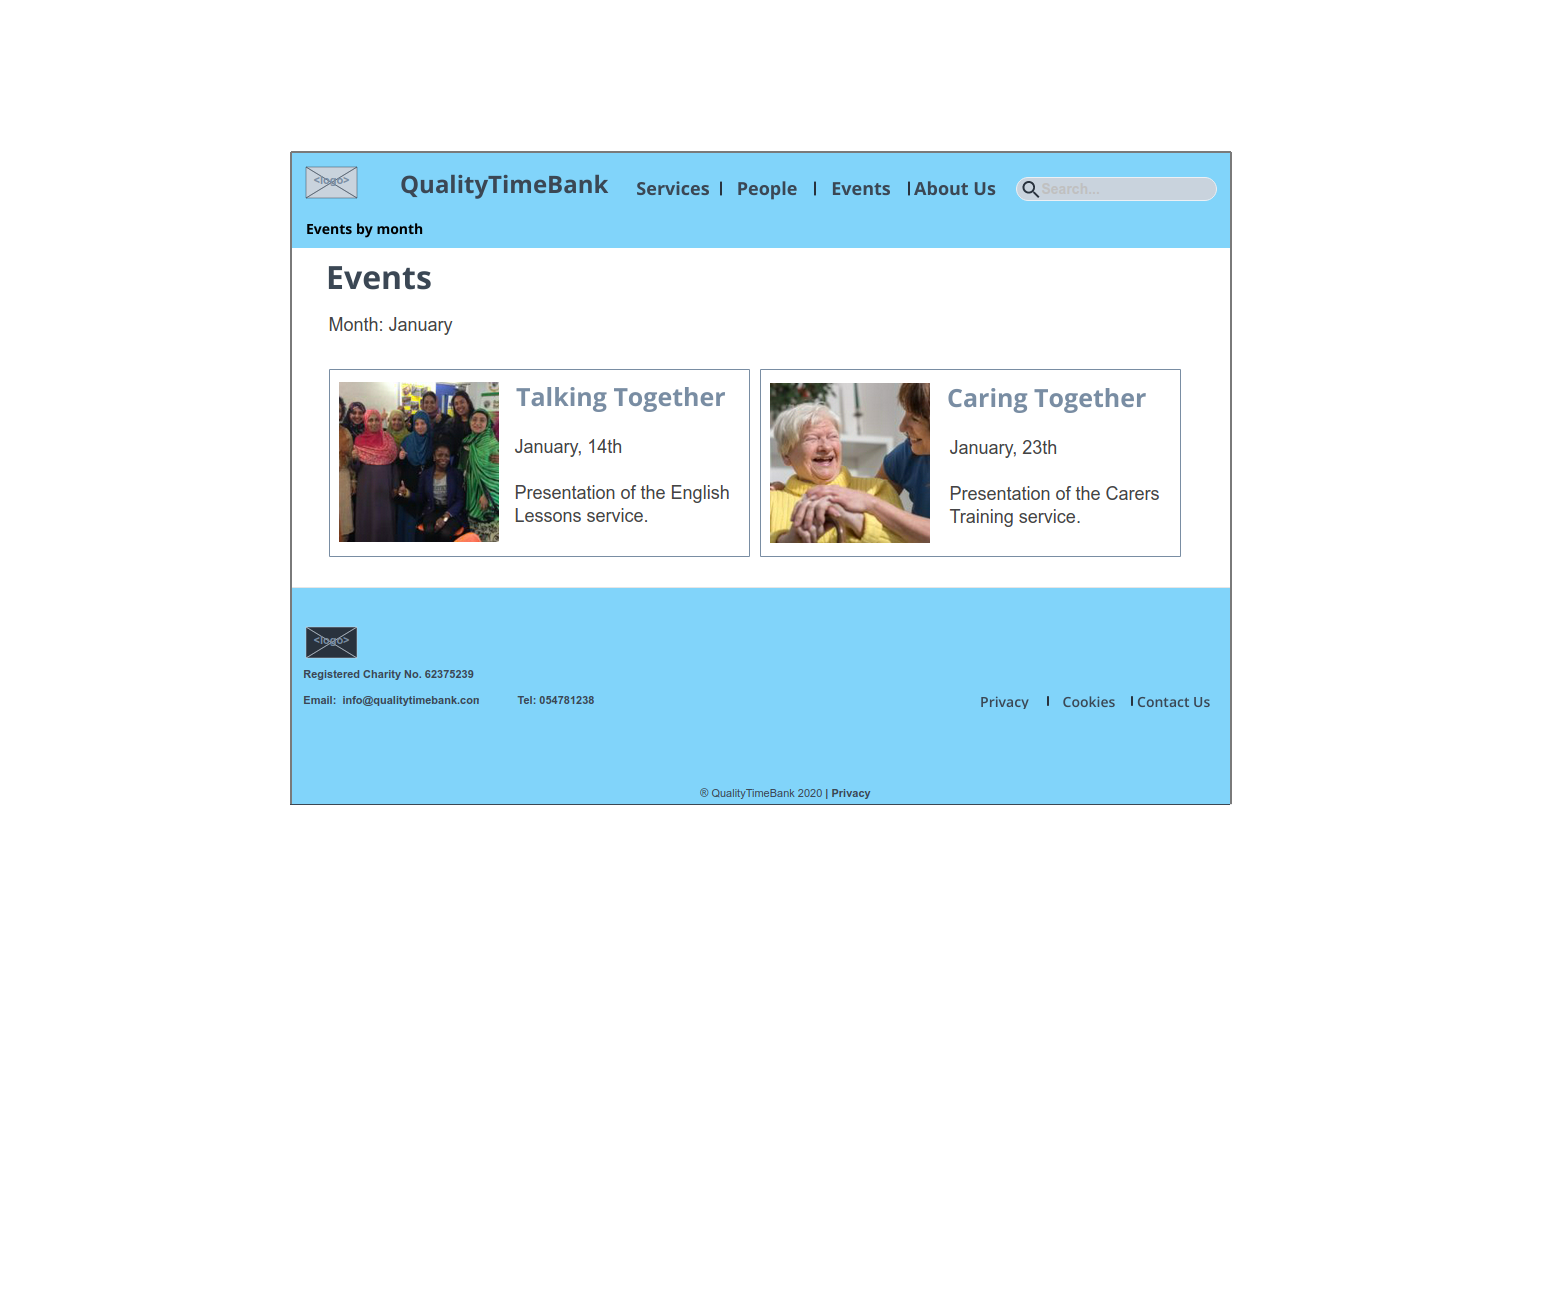
\includegraphics[width=1\linewidth, keepaspectratio]{mockups/ConcreteEventsJanuary}
    \caption{Mockup}
\end{figure}














\chapter{Database design}

\section{ER}

\begin{figure}[H]
    \centering
    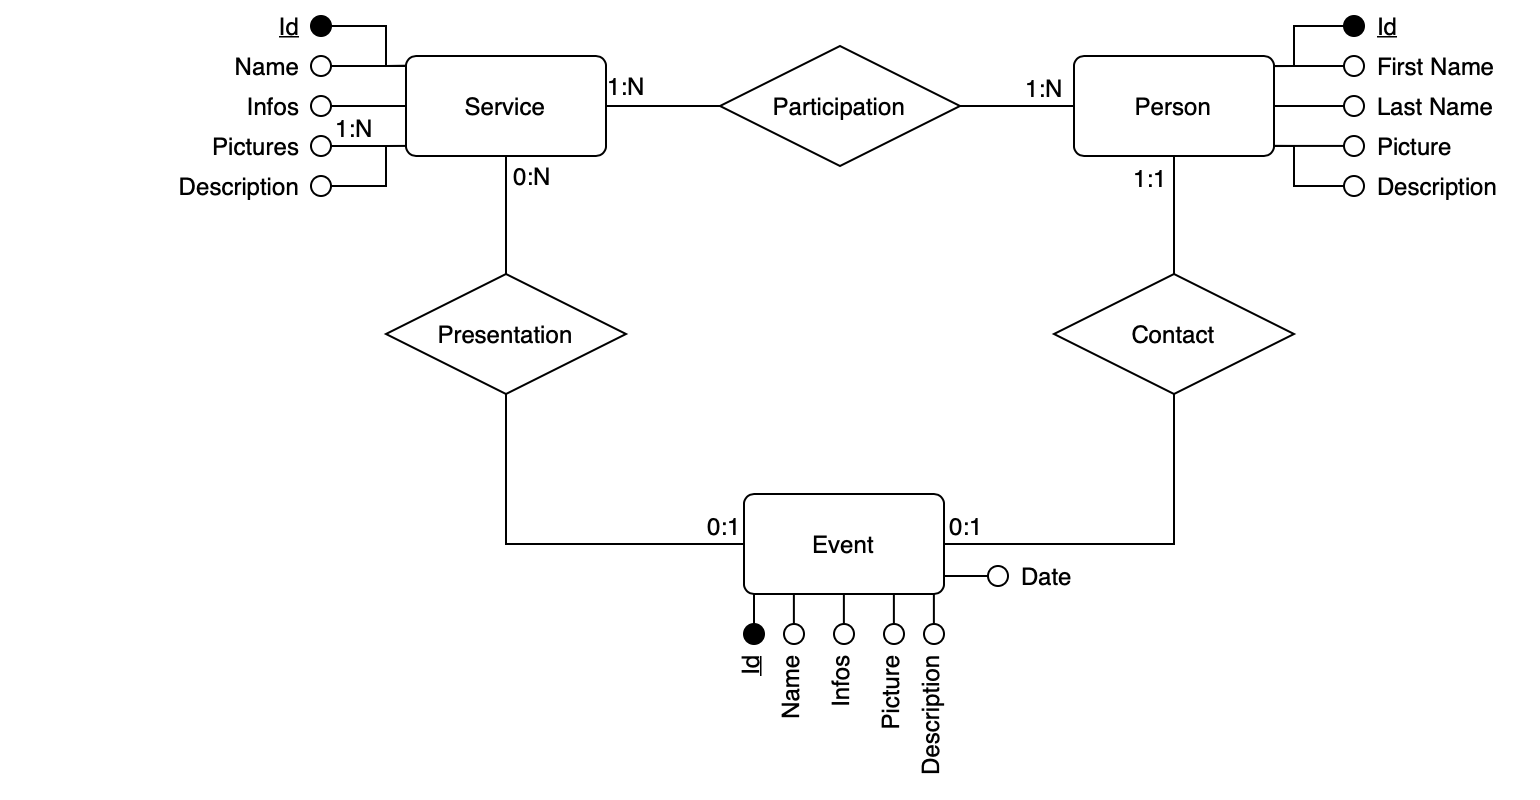
\includegraphics[width=0.72\linewidth, keepaspectratio]{DB/ER}
\end{figure}

\section{Relational tables}

\begin{figure}[H]
    \centering
    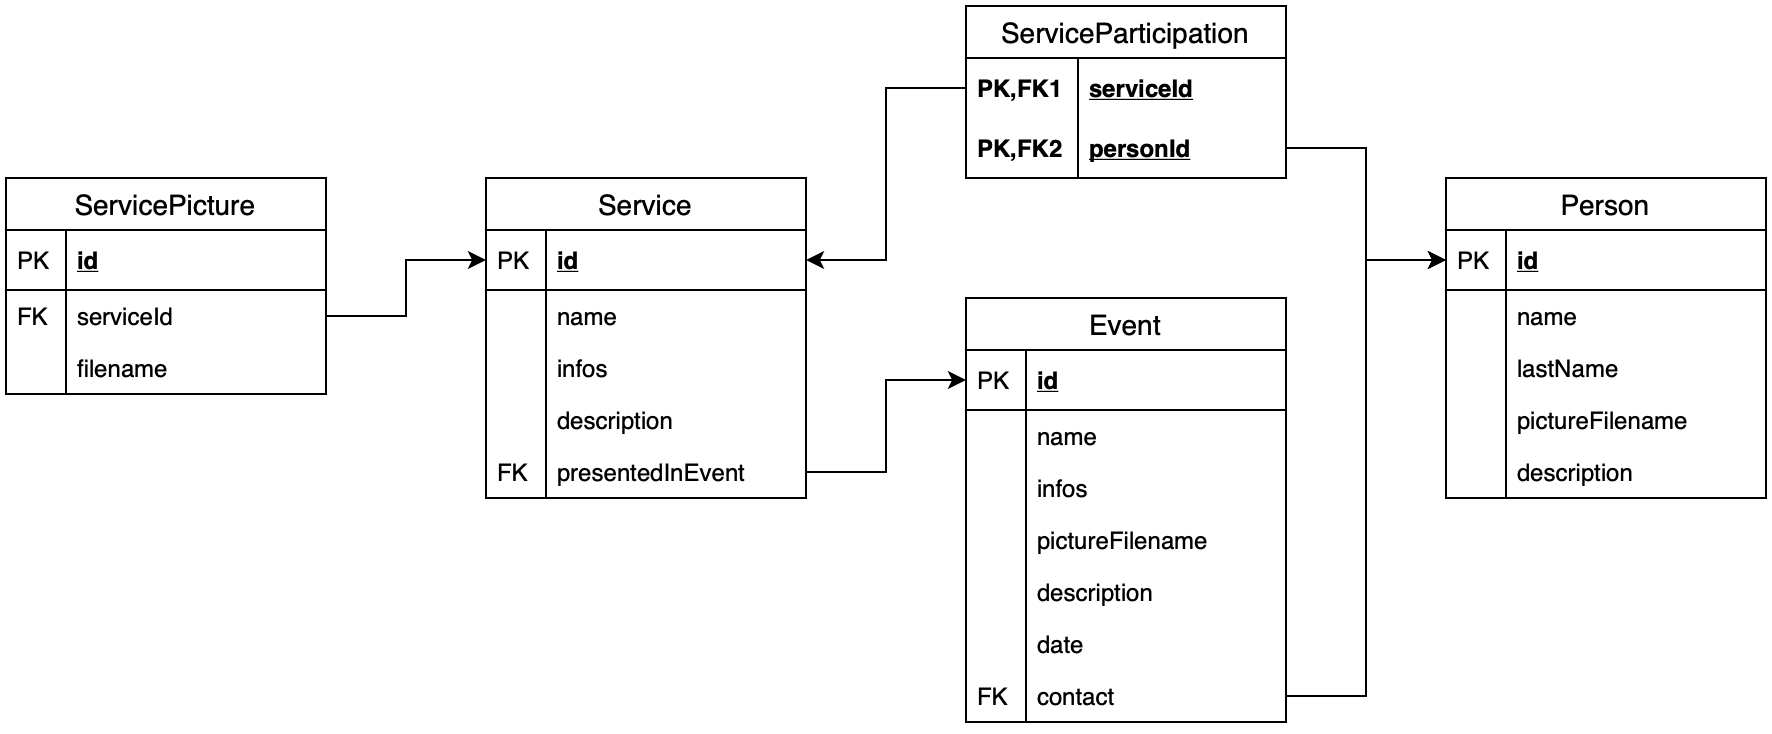
\includegraphics[width=0.72\linewidth, keepaspectratio]{DB/RelationalTables}
\end{figure}

\end{document}
